%%%%%%%%%%%%%%%%%%%%%%%%%%%%%%%%%%%%%%%%%%%%%%%%%%%%%%%%%%%%%%%%%%%%%%%%%%%%%%%%
% University of Western Ontario Thesis Template
% By: Justin Quinn Veenstra, 2010
% With thanks to Mr. (soon to be Dr.) Will Robertson.


\documentclass[12pt,twoside]{report}
\usepackage[acronym]{glossaries}
\makeglossaries
\usepackage{subcaption}
\captionsetup{compatibility=false}
\usepackage{minted}
\usepackage{xcolor} % to access the named colour LightGray

\newcommand\code{\texttt}
\newcommand\param{\textit}

%% Decomment next line to use PostScript fonts
%%\UsePackage{times}
%%%%%%%%%%%%%%%%%%%%%%%%%%%%%%%%%%%%%%%%%%%%%%%%%%%%%%%%%%%%%%%%%%%%%%%%
%%                                                                    %%
%%                    ***   I M P O R T A N T   ***                   %%
%%                                                                    %%
%% Fill in the following fields with the required information:        %%
%%  - \department{...}  name of the graduate department               %%
%%  - \degree{...}      name of the degree obtained                   %%
%%  - \author{...}      name of the author                            %%
%%  - \title{Three contributions to the theory and practice of optimizing compilers}       title of the thesis                           %%
%%  - \gyear{...}       year of graduation                            %%
%%  - \super{...}    supervisor
%%  - \firstname, \middlename, \lastname... there is additional documentation by the actual fields, so I'll leave it at that
%%%%%%%%%%%%%%%%%%%%%%%%%%%%%%%%%%%%%%%%%%%%%%%%%%%%%%%%%%%%%%%%%%%%%%%%
\usepackage{morewrites}
\usepackage{appendix}
\usepackage{graphicx,pifont,color} 
\usepackage{amsmath}
\usepackage[byname]{smartref}
%\usepackage{hyperref} %comment out for hardcopy

\usepackage{wrapfig}
\usepackage{txfonts}
\usepackage{tocloft}
\usepackage{paralist}
\usepackage[shortlabels]{enumitem}

\usepackage{hyperref}
\usepackage{lhelp}
\usepackage{listings}
\usepackage{float}

\usepackage{xcolor}
\lstset { %
	language=C,
	backgroundcolor=\color{black!5}, % set backgroundcolor
	basicstyle=\footnotesize,% basic font setting
	belowcaptionskip=1\baselineskip,
	breaklines=true,
	frame=L,
	xleftmargin=\parindent,
	showstringspaces=false,
	basicstyle=\footnotesize\ttfamily,
	keywordstyle=\bfseries\color{green!40!black},
	commentstyle=\itshape\color{purple!40!black},
	identifierstyle=\color{blue},
	stringstyle=\color{orange},
	numbers=left,
	stepnumber=1,
}

\usepackage{setspace}
\usepackage{subcaption}
%%\usepackage[pdftex]{graphicx} 
\usepackage{lhelp}
\usepackage{amsfonts,latexsym}
%%\usepackage{amsthm}
\usepackage{amsmath}
\usepackage{amssymb}
\usepackage{caption}
%\usepackage{MnSymbol}
\usepackage{verbatim}
\usepackage{tikz}
\usepackage{listings}
%%\usepackage{titlesec}
\usetikzlibrary{positioning,calc}
\usepackage{hyperref}
\usepackage{cleveref}
\usepackage{color}
\usepackage{subcaption}
\usepackage{animate}

\usepackage{booktabs}
\usepackage{multicol}
\usepackage{multirow}
\usepackage{tcolorbox}


%\usepackage{multicol}
%% plots, diagrams
\usepackage{float}
\usepackage{comment}
\usepackage{graphicx,pifont,color}
%\usepackage{algorithm}
\usepackage{algpseudocode}
\usepackage{hhline}
\usepackage{bm}
\usepackage{pgfplots}
\pgfplotsset{compat=1.10}
\usetikzlibrary{positioning,calc}
\usetikzlibrary{arrows.meta,chains,decorations.pathreplacing,scopes,positioning}
\usetikzlibrary{calc,shapes.multipart,chains,arrows}

%%%%%%%%%%%%%%%%%%%%%%%%%%
%%%% Mathematical Sets %%%
%%%%%%%%%%%%%%%%%%%%%%%%%%
%% \def\A{\mbox{${\mathbb A}$}}
\def\B{\mbox{${\mathbb B}$}}
\def\C{\mbox{${\mathbb C}$}}
\def\F{\mbox{${\mathbb F}$}}
%\def\H{\mbox{${\mathbb H}$}}
\def\K{\mbox{${\mathbb K}$}}
\def\N{\mbox{${\mathbb N}$}}
\def\Q{\mbox{${\mathbb Q}$}}
\def\R{\mbox{${\mathbb R}$}}
\def\Z{\mbox{${\mathbb Z}$}}

%%%%%%%%%%%%%%%%%%%%
%% Linear algebra %%
%%%%%%%%%%%%%%%%%%%%
\def\A {\ensuremath{\mathbf{A}}}
\def\BB {\ensuremath{\mathbf{B}}}
\def\CC {\ensuremath{\mathbf{C}}}
\def\D {\ensuremath{\mathbf{D}}}
\def\E {\ensuremath{\mathbf{E}}}
\def\G {\ensuremath{\mathbf{G}}}
\def\H {\ensuremath{\mathbf{H}}}
\def\M {\ensuremath{\mathbf{M}}}
\def\NN {\ensuremath{\mathbf{N}}}
\def\P {\ensuremath{\mathbf{P}}}
\def\QQ {\ensuremath{\mathbf{Q}}}
\def\S {\ensuremath{\mathbf{S}}}
\def\U {\ensuremath{\mathbf{U}}}
\def\V {\ensuremath{\mathbf{V}}}
\def\a {\ensuremath{\mathbf{a}}}
\def\b {\ensuremath{\vec{b}}}
\def\c {\ensuremath{\mathbf{c}}}
\def\d {\ensuremath{\mathbf{d}}}

\def\i {\ensuremath{\mathbf{i}}}
\def\j {\ensuremath{\mathbf{j}}}
\def\k {\ensuremath{\mathbf{k}}}
\def\m {\ensuremath{\mathbf{m}}}
\def\n {\ensuremath{\mathbf{n}}}
\def\p {\ensuremath{\mathbf{p}}}

\def\q {\ensuremath{\mathbf{q}}}
\def\t {\ensuremath{\mathbf{t}}}
\def\x {\ensuremath{\vec{x}}}
\def\u {\ensuremath{\mathbf{u}}}
\def\v {\ensuremath{\mathbf{v}}}
\def\w {\ensuremath{\mathbf{w}}}
\def\y {\ensuremath{\mathbf{y}}}
\def\z {\ensuremath{\mathbf{z}}}
\def\e {\ensuremath{\vec{e}}}
\def\0 {\ensuremath{\mathbf{0}}}
\newcommand{\Zero}[1]{\ensuremath{{\mathbf{0}}^{#1}}}
\newcommand{\rank}[1]{\ensuremath{{\rm rank}(#1)}}
\newcommand{\norm}[1]{\ensuremath{ \| {#1} \| }}



%%%%%%%%%%%%%%%%%%%%%%%%%%%%%%%%
%%% Computer algebra systems %%%
%%%%%%%%%%%%%%%%%%%%%%%%%%%%%%%%
\newcommand{\axiom}{\mbox{{\sc Axiom}}}
\newcommand{\axiomxl}{\mbox{{\sc AXIOM-XL}}}
\newcommand{\aldor}{\mbox{{\sc Aldor}}}
\newcommand{\gb}{\mbox{{\sc GB}}}
\newcommand{\basicmath}{\mbox{{\em BasicMath}}}
\newcommand{\aldorlib}{\mbox{{\em aldorlib}}}
\newcommand{\algebralib}{\mbox{{\em libalgbra}}}
\newcommand{\magma}{{\sc Magma}}
\newcommand{\maple}{{\sc Maple}}
\newcommand{\Maple}{{\sc Maple}}
\newcommand{\mathematica}{{\sc Mathematica}}
\newcommand{\matlab}{{\sc Matlab}}
\newcommand{\java}{{\sc Java}}
\newcommand{\pascal}{{\sc Pascal}}
\newcommand{\reduce}{{\sc Reduce}}
\newcommand{\singular}{{\sc Singular}}
\newcommand{\ntl}{\mbox{{\sc NTL}}}

%\def\language#1{\texttt{#1}}
\def\package#1{\textsc{#1}}
%\def\function#1{\textrm{#1}}
\def\userfunction#1{\textsf{#1}}
%\def\algorithm#1{\textsc{#1}}
\def\mathsymbol#1{\mbox{$#1$}}
%%\def\maple{\mbox{{\sc Maple}}}
%%\def\axiom{\mbox{{\sc AXIOM}}}
%%\def\aldor{\mbox{{\sc Aldor}}}
\def\fortran{\mbox{{\sc FORTRAN}}}
\def\scratchpad{{\tt scratchpad}}
%%\def\singular{\mbox{{\sc Singular}}}
\def\diffAlg{\mbox{{\sc DiffAlg}}}
\def\triade{\mbox{{\sc triade}}}
\def\kronecker{\mbox{{\tt Kronecker}}}
%% \def\delta{\mbox{{$\Delta$}}}
\def\Piit{\mbox{{${\Pi}^{it}$}}}
\def\sumit{\mbox{{${\Sigma}^{it}$}}}
\def\libaldor{\mbox{{\sc libaldor}}}
\def\libalgebra{\mbox{{\sc libalgebra}}}
\def\pardi{\mbox{{\sf Pardi}}}
\def\riff{\mbox{{\tt Riff}}}
\def\modpone{\mbox{{\tt modp1}}}
\def\modptwo{\mbox{{\tt modp2}}}
\def\recden{\mbox{{\tt recden}}}
\def\algebraic{\mbox{{\tt algebraic}}}

\def\RegularChains{\mbox{{\tt RegularChains}}}
\def\modpn{\mbox{{\tt modpn}}}
\def\cumodp{\mbox{{\tt CUMODP}}}
\def\bpas{\mbox{{\tt BPAS}}}
\def\ProgramAnalysis{\mbox{{\tt ProgramAnalysis}}}

\def\spiral{\mbox{\sc SPIRAL}}
\def\kaapi{\mbox{\sc Kaapi}}
\def\fasttriade{\mbox{\sc FastTriade}}
\def\cogepas{\mbox{\sc CoGePas}}
\def\pascolib{\mbox{{\sc PASCOLib}}}
\def\hpcsolve{\mbox{\sc HpcSolve}}
\def\cadyna{\mbox{\sc CADYNA}}

\newcommand{\cilk}{\mbox{\sc Cilk}}
\newcommand{\cilkview}{\mbox{\sc Cilkview}}
\newcommand{\cilkplus}{\mbox{\sc Cilkplus}}
\newcommand{\cilkp}{\mbox{\sc Cilk-P}}
\newcommand{\nvcc}{\mbox{\sc nvcc}}
\newcommand{\openmp}{\mbox{\sc OpenMP}}
\newcommand{\openmptasks}{\mbox{\sc OpenMP Tasks}}
\newcommand{\meta}{\mbox{\sc MetaFork}}
\newcommand{\ppcg}{\mbox{\sc PPCG}}
\newcommand{\ctocuda}{\mbox{\sc C-to-CUDA}}
\newcommand{\hicuda}{\mbox{\sc HiCUDA}}
\newcommand{\cudachill}{\mbox{\sc CUDA-CHiLL}}
\newcommand{\clang}{\mbox{\sc Clang}}
\newcommand{\llvm}{\mbox{\sc LLVM}}
\newcommand{\ptx}{\mbox{\sc PTX}}
\newcommand{\nvptx}{\mbox{\sc NVPTX}}
\newcommand{\tbb}{\mbox{\sc TBB}}
\newcommand{\openacc}{\mbox{\sc OpenACC}}
\newcommand{\opencl}{\mbox{\sc OpenCL}}
\newcommand{\cplusplusamp}{\mbox{\sc C++ AMP}}
\newcommand{\cuda}{\mbox{\sc CUDA}}
\newcommand{\gpu}{\mbox{\sc GPU}}
\newcommand{\ibmxl}{\mbox{\sc IBM XL}}


%% \bibliographystyle{abbrv} %% OK !!
%% \bibliographystyle{plain}
%% \bibliographystyle{apalike} %% KO 
%%\bibliographystyle{ieeetr} %% OK !
%% \bibliographystyle{siam}  %% KO 
%% \bibliographystyle{unsrt} %% OK !
%% \bibliographystyle{alpha}
%% \leftmargini=20pt

%%%%%%%%%%%%%%%%%%%%%%%%%
%%% Theorems and such %%%
%%%%%%%%%%%%%%%%%%%%%%%%%
%\newtheorem{corollary}{Corollary}
%\newtheorem{theorem}{Theorem}
%\newtheorem{lemma}{Lemma}
%\newtheorem{problem}{Problem}
%\newtheorem{definition}{Definition}
%\newtheorem{proposition}{Proposition}
%\newtheorem{notation}{Notation}
%\newtheorem{example}{Example}
%\newtheorem{hypothesis}{Hypothesis}
%\newtheorem{remark}{Remark}

%\algnewcommand\algorithmicswitch{\textbf{switch}}
%\algnewcommand\algorithmiccase{\textbf{case}}
%\algnewcommand\algorithmicassert{\texttt{assert}}
%\algnewcommand\Assert[1]{\State \algorithmicassert(#1)}%
% New "environments"
%\algdef{SE}[SWITCH]{Switch}{EndSwitch}[1]{\algorithmicswitch\ #1\ \algorithmicdo}{\algorithmicend\ \algorithmicswitch}%
%\algdef{SE}[CASE]{Case}{EndCase}[1]{\algorithmiccase\ #1}{\algorithmicend\ \algorithmiccase}%
%\algtext*{EndSwitch}%
%\algtext*{EndCase}%

%\newenvironment{Proof}{ {\noindent} {\sc Proof} $\rhd$}{$\lhd$}

%%%%%%%%%%%%%%%%%%%%%%%%%%%%%
%% Operations on polyhedra %%
%%%%%%%%%%%%%%%%%%%%%%%%%%%%%
\newcommand{\can}[1]{\mbox{{\sf can}$(#1)$}}
\newcommand{\proj}[1]{\mbox{{\sf proj}$(#1)$}}
\newcommand{\dproj}[1]{\mbox{{\sf Dproj}$(#1)$}}
\newcommand{\gproj}[1]{\mbox{{\sf Gproj}$(#1)$}}
\newcommand{\sol}[1]{\mbox{$V_{\Z}(#1)$}}

\newcommand{\isolve}[1]{\mbox{{\sf IntegerSolve}$(#1)$}}
\newcommand{\LP}[1]{\mbox{{\sf LP}$(#1)$}}



%%%%%%%%%%%%%%%%%%%%%%%%%%%%
%%% Miscellaneous macros %%%
%%%%%%%%%%%%%%%%%%%%%%%%%%%%
\newcommand{\hidetext}[1]{\mbox{ \ }}
\newcommand{\todo}[2]{{{\textcolor{red}{ #1}}}\footnote{ {\textcolor{blue}{ #2}} }}
\newcommand{\todolater}[2]{#1}
\newcommand{\fix}[3]{#1}
%% \newcommand{\reworked}[1]{{{\textcolor{blue}{ #1}}}}
\newcommand{\reworked}[1]{{ #1}}
\newcommand{\newfixed}[1]{{\color{black} #1}}

%%%%%%%%%%%%%%%%%%%%%%%%%%%%%%%%
%%% Computer algebra systems %%%
%%%%%%%%%%%%%%%%%%%%%%%%%%%%%%%%
\newcommand{\altran}{{\sc ALTRAN}}
\newcommand{\trip}{{\sc Trip}}
\newcommand{\pari}{{\sc Pari}}
\newcommand{\flint}{\mbox{{\sc FLINT}}}
\newcommand{\sympy}{\mbox{{\sc SymPy}}}
\newcommand{\cocoa}{\mbox{{\sc CoCoA}}}
\newcommand{\cocoalib}{\mbox{{\sc CoCoALib}}}
\newcommand{\symboliccpp}{\mbox{{\sc SymbolicC++}}}
\newcommand{\mmx}{\mbox{{\sc Mathemagix}}}
\newcommand{\linbox}{\mbox{{\sc LinBox}}}
\newcommand{\sage}{\mbox{{\sc SageMath}}}

\newcommand{\myproof}{\textsc{Proof.} }
\newcommand{\myfoorp}{\hfill$\square$}

\newcommand{\euclideanDivision}[4]{\mbox{{$ \begin{array}{c|c} #1 & #2 \\ \cline{2-2}
				#3 & #4 \\ \end{array} $}}}
%\newtheorem{Hypothesis}{Hypothesis}
%\newtheorem{Algorithm}{Algorithm}
%\newtheorem{theorem}{Theorem}
%\newtheorem{Lemma}{Lemma}
%\newtheorem{Corollary}{Corollary}
%\newtheorem{Conjecture}{Conjecture}
%\newtheorem{Proposition}{Proposition}
%\newtheorem{Definition}{Definition}
%\newtheorem{Notation}{Notation}
%\newtheorem{Example}{Example}
%\newtheorem{Remark}{Remark}
%\newtheorem{Problem}{Problem}
%\newtheorem{Acknowledgment}[]{Acknowledgment}
%\iffalse
%\newenvironment{proof}{\noindent{\em Proof:}}{$\Box$~\\}
%\fi
%%%%%%%%%%%%%%%%%%%%%%%%%%%%%%%%%%%%%%%%%%%%%
%% Math Symbol Macros
%%%%%%%%%%%%%%%%%%%%%%%%%%%%%%%%%%%%%%%%%%%%%
\def\B {\ensuremath{\mathbb{B}}}
%\def\A {\ensuremath{\mathbb{A}}}
\def\C {\ensuremath{\mathbb{C}}}
\def\I {\ensuremath{\mathcal{I}}}
\def\J {\ensuremath{\mathcal{J}}}
\def\K {\ensuremath{\mathbb{K}}}
\def\L {\ensuremath{\mathbb{L}}}
\def\N {\ensuremath{\mathbb{N}}}
\def\V {\ensuremath{\mathcal{V}}}
\def\W {\ensuremath{\mathcal{W}}}
\def\Q {\ensuremath{\mathbb{Q}}}
\def\R {\ensuremath{\mathbb{R}}}
\def\Z {\ensuremath{\mathbb{Z}}}
%\def\KK {\ensuremath{\overline{\mathbb{K}}}}

\newcommand{\T}{\mathfrak{T}}
%\newcommand{\G}{\mathcal{G}}
\renewcommand{\O}{\ensuremath{\mathcal{O}}}
\renewcommand{\o}{\ensuremath{\underline{o}}}

%%\def\u {\ensuremath{\mathbf{u}}}
%\def\U {\ensuremath{\underline{U}}}
\def\x {\ensuremath{\mathbf{x}}}
\def\X {\ensuremath{\underline{X}}}
\def\y {\ensuremath{\mathbf{y}}}
\def\Y {\ensuremath{\underline{Y}}}
\def\xx{\ensuremath{\underline{x}}}
\def\yy{\ensuremath{\underline{y}}}
\def\li{\ensuremath{\langle}}
\def\ri{\ensuremath{\rangle}}

%\newcommand{\NN}{\mbox{$N_{\geq}$}}
%\renewcommand{\PP}{\mbox{$P_{>}$}}
\newcommand{\HH}{\mbox{$H_{\neq}$}}
%\def\QQ {\ensuremath{\mathcal{Q}}}
\def\UU {\ensuremath{\mathcal{U}}}
%\def\VV {\ensuremath{\mathcal{V}}}

\newcommand{\limit}[1]{\mbox{${\lim}(#1)$}}

\renewcommand{\hat}[1]{\mbox{$\widehat{#1}$}}
\renewcommand{\tilde}[1]{\mbox{$ \overset{\thicksim}{#1} $}}



%%%%%%%%%%%%%%%%%%%%%%%%%%%%%%%%%%%%%%%%%%%%%
%% Polynomials and regular chains
%%%%%%%%%%%%%%%%%%%%%%%%%%%%%%%%%%%%%%%%%%%%%
\newcommand{\discrim}[1]{\mbox{{\rm discrim}$(#1)$}}
\newcommand{\init}[1]{\mbox{{\rm init}$(#1)$}}
\newcommand{\iter}[1]{\mbox{{\rm iter}$(#1)$}}
\newcommand{\mdeg}[1]{\mbox{{\rm mdeg}$(#1)$}}
\newcommand{\mvar}[1]{\mbox{{\rm mvar}$(#1)$}}
\newcommand{\prem}[1]{\mbox{{\rm prem}$(#1)$}}
\newcommand{\pquo}[1]{\mbox{{\rm pquo}$(#1)$}}
%\newcommand{\rank}[1]{\mbox{{\rm rank}$(#1)$}}
\newcommand{\ires}[1]{\mbox{{\rm ires}$(#1)$}}
\newcommand{\OpenCAD}[1]{\mbox{{\sf OpenCAD}$(#1)$}}
\newcommand{\OpenAugCAD}[1]{\mbox{{\sf OpenCAD}$(#1)$}}
\newcommand{\LazyRealTriangularize}[1]{\mbox{{\sf LazyRealTriangularize}$(#1)$}}
\newcommand{\GenerateFormula}[1]{\mbox{{\sf GenerateFormula}$(#1)$}}
\newcommand{\RealRootCounting}[1]{\mbox{{\sf RealRootCounting}$(#1)$}}
\newcommand{\ReviseFormula}[1]{\mbox{{\sf Disjunction}$(#1)$}}
\newcommand{\SamplePoints}[1]{\mbox{{\sf SamplePoints}$(#1)$}}
\newcommand{\factor}[1]{\mbox{{\sf factor}$(#1)$}}
\newcommand{\ProjectionFactorSet}[1]{\mbox{{\sf ProjectionFactorSet}$(#1)$}}
\newcommand{\notdone}{{\tt NotDone}}
\newcommand{\Intersect}[1]{\mbox{{\sf Intersect}$(#1)$}}
\newcommand{\GeneratePreRegularSas}[1]{\mbox{{\sf GeneratePreRegularSas}$(#1)$}}
\newcommand{\IteratedResultant}[1]{\mbox{{\sf res}$(#1)$}}
\newcommand{\IsolateBranchThroughOrigin}[1]{\mbox{{\sf IsolateBranchThroughOrigin}$(#1)$}}
\newcommand{\ExtractComponents}[1]{\mbox{{\sf ExtractComponents}$(#1)$}}
\newcommand{\LimitPoints}[1]{\mbox{{\sf LimitPoints}$(#1)$}}
\newcommand{\ChooseValues}[1]{\mbox{{\sf ChooseValues}$(#1)$}}
\newcommand{\RandomEllipsoid}[1]{\mbox{{\sf RandomEllipsoid}$(#1)$}}
\newcommand{\Minors}[1]{\mbox{{\sf Minors}$(#1)$}}
\newcommand{\hensel}[1]{\mbox{{\sf ExtendedHenselConstruction}$(#1)$}}
%\newcommand{\dim}[1]{\mbox{{\rm dim}$(#1)$}}


\newcommand{\Npoly}[1]{\mbox{$F^{(0)}(#1)$}}
\newcommand{\Gpoly}[1]{\mbox{$G^{(0)}(#1)$}}
\def\Z {\ensuremath{\mathbb{Z}}}
\newcommand{\ideal}[1]{\langle#1\rangle}
\usepackage{color, colortbl}
\definecolor{LRed}{rgb}{1,.8,.8}
\definecolor{MRed}{rgb}{1,.6,.5}
\definecolor{HRed}{rgb}{0.7,.5,.6}
\definecolor{HGray}{rgb}{0.8,.8,.8}
\definecolor{HGray2}{rgb}{0.9,.9,.9}
\definecolor{LBlue}{rgb}{0.8,1,1}

\newcolumntype{C}{>{\columncolor{LRed}}c}{\newcolumntype{C}{c}}
\newcolumntype{D}{>{\columncolor{MRed}}c}{\newcolumntype{D}{c}}
\newcolumntype{E}{>{\columncolor{HRed}}c}{\newcolumntype{E}{c}}
\newcolumntype{F}{>{\columncolor{HRed}}c}{\newcolumntype{F}{c}}
\newcolumntype{G}{>{\columncolor{HGray}}c}{\newcolumntype{G}{c}}
\usepackage{array}
\newcolumntype{?}{!{\vrule width 1pt}}

\newcommand{\xmark}{\ding{55}}

\newcommand{\EHC}[1]{\mbox{{\sf EHC\_Lift}$(#1)$}}
\newcommand{\MultTime}[1]{\mbox{${\mathsf M}(#1)$}}
\newcommand{\AlgExtTime}[1]{\mbox{${\sf A}(#1)$}}

\makeatletter
\providecommand*{\cupdot}{%
	\mathbin{%
		\mathpalette\@cupdot{}%
	}%
}
\newcommand*{\@cupdot}[2]{%
	\ooalign{%
		$\m@th#1\cup$\cr
		\hidewidth$\m@th#1\cdot$\hidewidth
	}%
}
\makeatother



\def\bpas{\mbox{{\tt BPAS}}}
\def\powerserieslib{\mbox{{\tt PowerSeries}}}

\newcommand{\cpp}{\mbox{C$++$}}

%%%%%%%%%%%%%%%%%%%%%%%%%%%%
%%% Miscellaneous macros %%%
%%%%%%%%%%%%%%%%%%%%%%%%%%%%

%% \newcommand{\reworked}[1]{{{\textcolor{blue}{ #1}}}}
\definecolor{nicedarkgreen}{rgb}{0.05, 0.35, 0.12}
\renewcommand{\gcd}[1]{\mbox{{\rm gcd}$(#1)$}}


%\newcommand{\reworked}[1]{{ #1}}
\newcommand{\alnam}[1]{\textsc{#1}}
\newcommand{\templ}[1]{$\langle$#1$\rangle$}
\newcommand{\vect}[1]{\boldsymbol{#1}}
\newcommand{\return}{\mathrm{\bf return}}
\newcommand{\OR}{\mathrm{\bf or}}
\newcommand{\AND}{\mathrm{\bf and}}
\newcommand{\TO}{\mathrm{\bf to}}
\newcommand{\textblockcomment}[1]{}
\renewcommand{\gets}{:=}

%%%%%%%%%%%%%%%%%%%%%%%%%%%
%%%%%%     red    %%%%%%%%%
%%%%%%%%%%%%%%%%%%%%%%%%%%%
%%\newcommand{\red}[1]{\textcolor{red}{ #1 }}
\newcommand{\red}[1]{{ #1 }}
\newcolumntype{?}{!{\vrule width 1pt}}

\newcommand{\mts}{ M }
\newcommand{\nmts}[1]{ M_{#1}}
\newcommand{\cG}{\mathcal{D}}
\newcommand{\cC}{\mathcal{C}}
%\newcommand{\vv}[1]{v\!\brac{#1}}
\renewcommand{\ss}{\vec{s}}
\newcommand{\sO}{\mathcal{O}}
\newcommand{\sC}{\mathcal{C}}

\newcommand{\nts}[1]{\vec{t}_{#1}}
\newcommand{\LLs}[1]{\vec{L}_{#1}}
\newcommand{\xdim}[2]{{\rm dim}_{#1}\hspace{-.1em}\brac{#2}}
\newcommand{\height}[1]{{\rm height}\hspace{-.1em}\brac{#1}}

%\newcommand{\xdim}[1]{\underset{\textrm{vec}}{\textrm{dim}}\left(#1\right)}
\DeclareMathOperator*{\DIM}{dim}
\newcommand{\vdim}[1]{\DIM_{\text{vec}}(#1)}

%\newcommand{\limit}[1]{\mbox{${\lim}(#1)$}}

\newcommand{\xdeg}[2]{{\rm deg}_{#2}\brac{#1}}
\newcommand{ \transverse }{ \pitchfork } 
%\newcommand{\im}[2]{{\rm im}\hspace{-.1em}\brac{#1;\,#2}}		% Intersection Multiplicity
%\newcommand{\imN}[3]{{\rm im}_{#1}\hspace{-.1em}\brac{\,#2;\,#3}}		% Intersection Multiplicity
%\newcommand{\ims}[3]{{\rm im}_{#1}^{\ast}\hspace{-.1em}\brac{\,#2;\,#3}}		% Intersection Multiplicity
\newcommand{\im}[2]{{\rm IM}\hspace{-.1em}\brac{#1;\,#2}} 			%Intersection Multiplicity
\newcommand{\imt}[2]{{\rm im_2}\hspace{-.1em}\brac{#1;\,#2}}
\newcommand{\mt}[2]{{\rm m}_{#1}(#2)}	%multiplicity
\newcommand{\imn}[3]{{\rm im_{#1}}\hspace{-.1em}\brac{#2;\,#3}}
\newcommand{\NF}[2]{{\rm NF}\hspace{-.1em}\brac{#1,\,\ideal{#2}}}  %Normal form
\newcommand{\nf}[2]{{\rm NF}\hspace{-.1em}\brac{#1,\,#2}}    %Normal form
\newcommand{\Regularize}[2]{{\rm Regularize}\hspace{-.1em}\brac{#1,\,\ideal{#2}}}
\newcommand{\regularize}[2]{{\rm Regularize}\hspace{-.1em}\brac{#1,\,#2}}


%logic
\renewcommand{\lor}{~{\rm or }}
\newcommand{\lxor}{~{\rm xor }}
\renewcommand{\land}{~{\rm and }}
\newcommand{\bor}{\mathbf{or}}
\newcommand{\band}{\mathbf{and}}

%regular chains
\newcommand{\TT}{\vec{T}}
%\newcommand{\ts}{\vec{t}}
%\newcommand{\init}[1]{\mbox{${\rm init}\!\brac{#1}$}}
%\newcommand{\sat}[2]{#1 \colond #2^\infty}
%%\newcommand{\isat}[1]{{\rm sat}\!\brac{#1}}
\newcommand{\isat}[1]{\mbox{{\rm sat}$(#1)$}}

%polynomials
\newcommand{\tsetsof}[1]{\mathbb{T}\brac{#1}}
\newcommand{\termsof}[1]{{\rm terms}\brac{#1}}
\newcommand{\monosof}[1]{{\rm monos}\brac{#1}}
\newcommand{\indetsof}[1]{{\rm indets}\brac{#1}}
\newcommand{\lc}[1]{{\rm lc}({#1})}
\newcommand{\xlc}[2]{\ell\hspace{-.1em}{\it c}_{#2}\brac{#1}}
\newcommand{\lt}[1]{\ell\hspace{-.1em}{\it t}\brac{#1}}
\newcommand{\xlt}[2]{\ell\hspace{-.1em}{\it t}_{#2}\brac{#1}}
\newcommand{\lm}[1]{\ell\hspace{-.1em}{\it m}\brac{#1}}
\newcommand{\xlm}[2]{\ell\hspace{-.1em}{\it m}_{#2}\brac{#1}}

%bracketing
\newcommand{\lbrac}[1]{\sbrac{\,#1\,}}
\newcommand{\cbrac}[1]{\left\{ #1 \right\}}
\newcommand{\brac}[1]{\left( #1 \right)}
\newcommand{\abs}[1]{\left| #1 \right|}
\newcommand{\kvs}[2]{ \langle\hspace{-.1em}\langle\, #1 \,\rangle\hspace{-.1em}\rangle}
%\newcommand{\ideal}[1]{\left<\hspace{.1em} #1 \hspace{.1em}\right >}
\newcommand{\sideal}[1]{\langle\, #1 \,\rangle}

%algebraic geometry
\newcommand{\VV}[1]{\mathbf{V}\hspace{-.1em}\brac{#1}}  % Variety
\def \V {\mathbf{V}}
%\newcommand{\WW}[1]{\mathbf{W}\hspace{-.1em}\brac{#1}}  % Quasi Component
\def \WW {\mathbf{W}}
\newcommand{\II}[1]{\mathbf{I}\hspace{-.1em}\brac{#1}}  % Ideal
%% \newcommand{\tcone}[2]{ \mbox{\large $\kappa$}_{#1}\brac{#2} }
\newcommand{\tcone}[2]{ TC_{#1}\!\brac{#2} }
\newcommand{\tplane}[2]{ \mbox{ $\mathbf{d}$}_{#1}\brac{#2} }
\newcommand{\tspace}[2]{ T_{#1}\!\brac{#2} }
\newcommand{\cspace}[2]{ TC_{#1}\!\brac{#2} }
\newcommand{\tline}{ \mbox{\large $\lambda$} }
\newcommand{\sing}[1]{{\rm sing}\hspace{-.1em}\brac{#1}}
\let\iso\cong
\renewcommand{\cong}{\equiv}
%\renewcommand{\mod}{\,\mathbin{\rm mod}}
\newcommand{\rem}{\,\mathbin{\rm rem}}
%\newcommand{\prem}{\,\mathbin{\rm prem}}
\def\mymathhyphen{{\hbox{-}}}


%calculus
\newcommand{\jac}[1]{\text{jac}\brac{#1}}
\newcommand{\syl}[3]{\text{syl}\brac{#1,\,#2,\,#3}}
\newcommand{\env}[1]{\text{env}\brac{#1}}
\newcommand{\grad}[1]{\nabla\brac{#1}}
\newcommand{\pdiff}[2]{\frac{\partial #1}{\partial #2}}
\newcommand{\hc}[3]{\textsc{hc}_{#3}\brac{#1;\,#2}}


%standard sets
\newcommand{\ZZ}{\mathbb{Z}}   % Integers
\newcommand{\RR}{\mathbb{R}}   % Reals
\newcommand{\KK}{\mathbb{K}}   % Reals
%\newcommand{\PP}{\mathbb{P}}   % Projective space
\renewcommand{\AA}{\mathbb{A}} % Affine space

\newcommand{\kk}{\KK}
\newcommand{\hh}{\vec{h}}
\newcommand{\ff}{\vec{t}}
%\newcommand{\xx}{\vec{x}}
\newcommand{\mm}{\vec{m}}
%\newcommand{\yy}{\vec{y}}
\newcommand{\ii}{{\rm I}}
\newcommand{\LL}{\mathbf{L}}

%\newcommand{\mod}{$\ $ {\sf mod}}
\newcommand{\moddeg}[2]{\mbox{${\rm moddeg} (#1,#2 )$}}
\newcommand{\tdeg}[2]{\mbox{${\rm deg} (#1,#2 )$}}

%IM
%\newcommand{\im}[1]{${\sf I} (#1)$}
%\newcommand{\IM}[2]{${\sf IM} {#1}(#2)$}
\newcommand{\quo}{\text{quo}}

\def\HiLiYellow{\leavevmode\rlap{\hbox to \hsize{\color{yellow!}\leaders\hrule height .8\baselineskip depth .5ex\hfill}}}
\def\HiLiRed{\leavevmode\rlap{\hbox to \hsize{\color{red!}\leaders\hrule height .8\baselineskip depth .5ex\hfill}}}
\def\HiLiBlue{\leavevmode\rlap{\hbox to \hsize{\color{cyan!}\leaders\hrule height .8\baselineskip depth .7ex\hfill}}}
\def\HiLiGreen{\leavevmode\rlap{\hbox to \hsize{\color{green!}\leaders\hrule height .8\baselineskip depth .5ex\hfill}}}
\def\HiLiPink{\leavevmode\rlap{\hbox to \hsize{\color{pink!}\leaders\hrule height .8\baselineskip depth .5ex\hfill}}}
\def\HiLiOrange{\leavevmode\rlap{\hbox to \hsize{\color{orange!}\leaders\hrule height .8\baselineskip depth .5ex\hfill}}}
\def\HiLiPurple{\leavevmode\rlap{\hbox to \hsize{\color{violet!}\leaders\hrule height .8\baselineskip depth .5ex\hfill}}}
\def\HiLiGrey{\leavevmode\rlap{\hbox to \hsize{\color{lightgray!}\leaders\hrule height .8\baselineskip depth .5ex\hfill}}}
\def\HiLiGreyB{\leavevmode\rlap{\hbox to \hsize{\color{lightgray!}\leaders\hrule height .8\baselineskip depth 1.0ex\hfill}}}
\def\HiLiOlive{\leavevmode\rlap{\hbox to \hsize{\color{olive!}\leaders\hrule height .8\baselineskip depth .5ex\hfill}}}
\def\HiLiTeal{\leavevmode\rlap{\hbox to \hsize{\color{teal!}\leaders\hrule height .8\baselineskip depth .5ex\hfill}}}
\def\HiLiLime{\leavevmode\rlap{\hbox to \hsize{\color{lime!}\leaders\hrule height .8\baselineskip depth .5ex\hfill}}}

\newcommand{\hilightyellow}[1]{\colorbox{yellow}{#1}}
\newcommand{\hilightblue}[1]{\colorbox{cyan}{#1}}
\newcommand{\hilightred}[1]{\colorbox{red}{#1}}
\newcommand{\hilightgreen}[1]{\colorbox{green}{#1}}

%%%%%%%%%%%%%%%%%%%%%
%% Delinearization %%
%%%%%%%%%%%%%%%%%%%%%

\def\i {\ensuremath{\mathbf{i}}}
\def\j {\ensuremath{\mathbf{j}}}
\def\k {\ensuremath{\mathbf{k}}}
\def\m {\ensuremath{\mathbf{m}}}
\def\n {\ensuremath{\mathbf{n}}}
\def\p {\ensuremath{\mathbf{p}}}

\newcommand{\iii}[1]{\mbox{${\mathbf{i}_{#1}}$}}
\newcommand{\mmm}[1]{\mbox{${\mathbf{m}_{#1}}$}}
\newcommand{\pp}[1]{\mbox{${\mathbf{p}_{#1}}$}}
\newcommand{\rr}[1]{\mbox{${\mathbf{r}_{#1}}$}}
\newcommand{\MMM}[1]{\mbox{${\mathbf{M}_{#1}}$}}


\usepackage{animate}
\usetikzlibrary{patterns}
\tikzset{every path/.style=thick}
\usepackage{pgfplots}
\usepgfplotslibrary{polar}
\usepgflibrary{shapes.geometric}
\usetikzlibrary{calc}
\pgfplotsset{my style/.append style={axis x line=middle, axis y line=
		middle, xlabel={$x$}, ylabel={$y$}, axis equal }}
\usepackage[linesnumbered,ruled,vlined]{algorithm2e}
%
%\usepackage{utopia}
%\usepackage{charter}
%\usepackage{pifont}
%mathptmx, helvet, avat, bookman, 
%chancery, charter, culer, mathtime, 
%mathptm, newcent, palatino, pifont,
%utopia.
%\usefonttheme{professionalfonts} % using non standard fonts for beamer
%\usepackage{fontspec}
    %setting a font
%\setsansfont{Adobe Garamond Pro}

%\setmainfont{Adobe Garamond Pro}
%   
%\usefonttheme[stillsansseriflarge]{serif}
%\usefonttheme{default}


%\usepackage{tgbonum}
%\usepackage[left=1in, right=1in, top=0.5in, bottom=1in]{geometry}

\usepackage{listings}
\usepackage{color}
\usepackage{verbatim}
\usepackage{fancyvrb}
\usepackage{lhelp}
\usepackage{xcolor}
%\usepackage[table, svgnames, dvipsnames]{xcolor}

\usepackage{hyperref} %comment out for hardcopy
\hypersetup{
	colorlinks,
	linkcolor={blue!50!black},
    citecolor={blue!50!black},
    urlcolor={blue!80!black}
   }

\newif\ifcomment
\commentfalse


%\usepackage [english]{babel}
%\usepackage [autostyle, english = american]{csquotes}
%\MakeOuterQuote{"}

%\usepackage[T1]{fontenc}
%\usepackage{textcomp}
%\usepackage [english]{babel}
%\usepackage [autostyle, english = american]{csquotes}
%\MakeOuterQuote{"}

\usepackage{pgfplots}
\pgfplotsset{compat=1.13}
%%%%%%%%%%%%%%%%%%%%%%%%%%%%%%%%%%%%
\pgfkeys{
     /pgf/number format/precision=2, 
    /pgf/number format/fixed zerofill=true,
    /pgf/number format/fixed
}
%%%%%%%%%%%%%%%%%%%%%%%%%%%%%%%%%%%%

\usepackage{tikz}
\usetikzlibrary{patterns}
%\usetikzlibrary{shadows.blur}

%\usepackage{helvet}
%\usepackage{fontspec}

%\usepackage{xcolor}
%\newcommand\code{{\fontsize{8}{8}$\#$}\fontfamily=\ttfamily \fontsize{8}{8}\selectfont}
\newcommand\term{{\fontsize{8}{8}}\fontfamily=\ttfamily \fontsize{8}{8}\selectfont}

%\setlist[itemize]{noitemsep, topsep=0pt}
%%\setlist[itemize]{itemsep=0.05pt, topsep=0pt}
%\setlist[enumerate]{noitemsep, topsep=0pt}
%\setlist[enumerate]{itemsep=0.2pt, topsep=0pt}

\let\oldcenter\center
\let\oldendcenter\endcenter
\renewenvironment{center}{\setlength\topsep{0pt}\oldcenter}{\oldendcenter}

%\renewcommand{\baselinestretch}{1.2}
\setlength{\parindent}{0pt}
\setlength{\parskip}{1.3ex}
\usepackage[nodisplayskipstretch]{setspace}
%\setstretch{1.4}
\setlength{\leftmargini}{8pt}
%\addtobeamertemplate{block begin}{%
%  \setlength{\textwidth}{1.2\textwidth}%
%}{}


\setlength{\textfloatsep}{0.075em}% Remove \textfloatsep
\setlength{\floatsep}{0.025ex}% Remove \textfloatsep
\setlength{\intextsep}{0.025em}% Remove \textfloatsep


\setlength{\belowcaptionskip}{0.5em}

\usepackage{algorithm}
%\usepackage[ruled,vlined,linesnumbered]{algorithm2e}
%\usepackage{algorithmicx}
\usepackage{algcompatible}
\usepackage{algpseudocode}

\algrenewcommand\algorithmicend{\textsf{\textbf{end}}}
\algrenewcommand\algorithmicdo{\textsf{\textbf{do}}}
\algrenewcommand\algorithmicwhile{\textsf{\textbf{while}}}
\algrenewcommand\algorithmicfor{\textsf{\textbf{for}}}
\algrenewcommand\algorithmicforall{\textsf{\textbf{for all}}}
\algrenewcommand\algorithmicloop{\textsf{\textbf{loop}}}
\algrenewcommand\algorithmicrepeat{\textsf{\textbf{repeat}}}
\algrenewcommand\algorithmicuntil{\textsf{\textbf{until}}}
\algrenewcommand\algorithmicprocedure{\textsf{\textbf{procedure}}}
\algrenewcommand\algorithmicfunction{\textsf{\textbf{function}}}
\algrenewcommand\algorithmicif{\textsf{\textbf{if}}}
\algrenewcommand\algorithmicthen{\textsf{\textbf{then}}}
\algrenewcommand\algorithmicelse{\textsf{\textbf{else}}}
\algrenewcommand\algorithmicrequire{\textsf{\textbf{Require:}}}
\algrenewcommand\algorithmicensure{\textsf{\textbf{Ensure:}}}
\algrenewcommand\algorithmicreturn{\textsf{\textbf{return}}}

\usepackage{caption}

% primary blue 33 7a b7
% info blue 31 70 8f

%\definecolor{wp}{rgb}{0.29,0.14,0.47}
%\definecolor{wpbright}{rgb}{0.58,0.45,0.74}

\definecolor{wp}{rgb}{0.129,0.478, 0.678}
%\definecolor{wp}{rgb}{0.26,0.55, 0.79}
%\definecolor{wpbright}{rgb}{0.192, 0.439, 0.561}\\
%\definecolor{wpbright}{rgb}{0.43, 0.43, 0.43}
%\definecolor{wp}{rgb}{0.19, 0.45, 0.66}
\definecolor{wpbright}{rgb}{0.26,0.55, 0.79}

\definecolor{yellowBright}{HTML}{FFD247}
\definecolor{orangeBright}{HTML}{FF7E47}
\definecolor{gray1}{HTML}{CEDBE1}
\definecolor{gray2}{HTML}{DDE6EA}
\definecolor{gray3}{HTML}{E3E6EB}
\definecolor{darkblue1}{HTML}{2375B9}%{0A599B}
\definecolor{darkblue2}{HTML}{3D577A}
\definecolor{lightblue1}{HTML}{65A4D9}
\definecolor{lightblue2}{HTML}{94C3E9}
\definecolor{red1}{HTML}{E4001B}
\definecolor{red2}{HTML}{8F2831}
\definecolor{lime1}{HTML}{AEBD63}
\definecolor{navy}{HTML}{000063}
\definecolor{pistachio}{HTML}{99CC66}
\definecolor{burgundy}{HTML}{900020}
\definecolor{coolgrey}{HTML}{8c92ac}
\definecolor{green1}{HTML}{A4C639}
\definecolor{byzantium}{HTML}{702963}
\definecolor{pastelgreen}{HTML}{03c03c}

\definecolor{purple1}{HTML}{8F2831}
\definecolor{contrast}{HTML}{CE0000}
%\colorlet{mycolor}{someothercolor}

\definecolor{positive}{HTML}{0D900F}
\definecolor{negative}{HTML}{FF0000}

\definecolor{dNone}{HTML}{FFFFFF}
%\definecolor{dOne}{HTML}{yellow}
%\definecolor{dTwo}{HTML}{blue}
%\definecolor{dThree}{HTML}{green}
%\definecolor{dFour}{HTML}{red}
\colorlet{dOne}{coolgrey!70}
\colorlet{dTwo}{pistachio!70}
\colorlet{dThree}{lightblue1!70}
\colorlet{dFour}{negative!70}

\colorlet{dOneLight}{dOne!40}
\colorlet{dTwoLight}{dTwo!40}
\colorlet{dThreeLight}{dThree!40}
\colorlet{dFourLight}{dFour!40}




%%%%%%%%%%%%%%%%%%%%%%%%%%%%%%%%%%%%%%%%%%%%%%%%%%
%\newcommand{\zpz}{$\mathbb{Z}/p\mathbb{Z}$}
%\newcommand{\mz}{$\mathbb{Z}$}
%\newcommand{\Z}{\mathbb{Z}}
%\newcommand{\Q}{\mathbb{Q}}
%\newcommand{\local}{\texttt{{\bf local: }}}
%\newcommand{\tid}{\local {\texttt{tid := blockIdx.x$*$blockSize.x$+$threadIdx.x}}}
%\newcommand{\mword}{of a machine-word}
%\newcommand{\initzero}{all digits initially set to 0}
%\newcommand{\algskeleton}{Template}
%\newcommand{\changeToAlgSkeleton}{
%\renewcommand{\thealgorithm}{}
%%	\renewcommand{\thealgorithm}{}
%	\renewcommand{\addcontentsline}[3]{}
%	\floatname{algorithm}{\algskeleton}
%	}
%\newcommand{\twiddle}[2]{D_{K,{#1}}}
%\def\DFT{\ensuremath{\mathrm{DFT}}}
%\newcommand{\cumodp}{CUMODP}
%
%\def\DFT{\ensuremath{\mathrm{DFT}}}
%\def\xx{\ensuremath{\mathbf{x}}}
%\def\yy{\ensuremath{\mathbf{y}}}
%%%%%%%%%%%%%%%%%%%%%%%%%%%%%%%%%%%%%%%%%%%%%%%%%%



%\newcolumntype{redcolor}{>{\columncolor{red}}c}

\newenvironment{proof}[1][Proof]{\begin{trivlist}
		\item[\hskip \labelsep {\bfseries #1}]}{\end{trivlist}}
\newenvironment{remark}[1][Remark]{\begin{trivlist}
		\item[\hskip \labelsep {\bfseries #1}]}{\end{trivlist}}

\newif\ifoldversion
\oldversionfalse

\newif\iflongversion
\longversionfalse

%\setlist{nosep} % or 
%\setlist{noitemsep}%	 to leave space around whole list
%
%\setlength{\intextsep}{1ex}
%\setlength{\textfloatsep}{1ex}
%\setlength{\floatsep}{1pt}
\setlist[itemize]{noitemsep, topsep=0pt}
%\setlist[itemize]{itemsep=0.05pt, topsep=0pt}
\setlist[enumerate]{noitemsep, topsep=0pt}
%\setlist[enumerate]{itemsep=0.2pt, topsep=0pt}
\makeatletter
\numberwithin{figure}{chapter}
\newenvironment{acknowledgements}%
{\clearemptydoublepage
 \begin{center}
  \section*{Acknowledgements}
 \end{center}
 \begingroup
}{\newpage\endgroup}

\newenvironment{dedication}%
{\clearemptydoublepage 
 \begin{center}
  \section*{Dedication}
 \end{center}
 \begingroup
}{\newpage\endgroup}

\newenvironment{preliminary}%
{\pagestyle{plain}\pagenumbering{roman}}%
{\pagenumbering{arabic}}

\addtoreflist{chapter}


\usepackage{caption}% http://ctan.org/pkg/caption
%\captionsetup[ruled]{labelsep=period}
%\makeatletter
%\@addtoreset{algorithm}{chapter}% algorithm counter resets every chapter
%\makeatother
%\renewcommand{\thealgorithm}{\thechapter.\arabic{algorithm}}% Algorithm # is <chapter>.<algorithm>\\

\let\savedCaption=\caption
\renewcommand{\caption}[1]{
	\savedCaption{\small #1}
}

% Default values for title page.

%% To produce output with the desired line spacing, the argument of
%% \spacing should be multiplied by 5/6 = 0.8333, so that 1 1/2 spaced
%% corresponds to \spacing{1.5} and double spaced is \spacing{1.66}.
\def\normalspacing{1.25} % default line spacing


%% Define the "thesis" page style.
\if@twoside % If two-sided printing.
\def\ps@thesis{\let\@mkboth\markboth
   \def\@oddfoot{}
   \let\@evenfoot\@oddfoot
   \def\@oddhead{
      {\sc\rightmark} \hfil \rm\thepage
      }
   \def\@evenhead{
      \rm\thepage \hfil {\sc\leftmark}
      }
   \def\chaptermark##1{\markboth{\ifnum \c@secnumdepth >\m@ne
      Chapter\ \thechapter. \ \fi ##1}{}}
   \def\sectionmark##1{\markright{\ifnum \c@secnumdepth >\z@
      \thesection. \ \fi ##1}}}
\else % If one-sided printing.
\def\ps@thesis{\let\@mkboth\markboth
   \def\@oddfoot{}
   \def\@oddhead{
      {\sc\rightmark} \hfil \rm\thepage
      }
   \def\chaptermark##1{\markright{\ifnum \c@secnumdepth >\m@ne
      Chapter\ \thechapter. \ \fi ##1}}}
\fi

\pagestyle{thesis}
% Set up page layout.
\setlength{\textheight}{9in} % Height of the main body of the text
\setlength{\topmargin}{-.5in} % .5" margin on top of page
\setlength{\headsep}{.5in}  % space between header and top of body
\addtolength{\headsep}{-\headheight} % See The LaTeX Companion, p 85
\setlength{\footskip}{.5in}  % space between footer and bottom of body
\setlength{\textwidth}{6.25in} % width of the body of the text
\setlength{\oddsidemargin}{.25in} % 1.25" margin on the left for odd pages
\setlength{\evensidemargin}{0in} % 1.25"  margin on the right for even pages

% Marginal notes
\setlength{\marginparwidth}{.75in} % width of marginal notes
\setlength{\marginparsep}{.125in} % space between marginal notes and text

% Make each page fill up the entire page. comment this out if you
% prefer. 
\flushbottom

\setcounter{tocdepth}{3} % Number the subsubsections 
\def\normalspacing{1.25} % default line spacing

\newcommand\isco[1]{%
  \edef\@tempa{#1}%
  \def\@tempb{}%
  \ifx\@tempa\@tempb
	\else \\\underline{Co-Supervisor:}\vspace{0.35in}\\\dots\dots\dots\dots\dots\dots\dots\\{#1}\\
  \fi
}

\newcommand\isjoint[1]{%
  \edef\@tempa{#1}%
  \def\@tempb{}%
  \ifx\@tempa\@tempb
	\else \\\underline{Joint Supervisor:}\vspace{0.35in}\\\dots\dots\dots\dots\dots\dots\dots\\{#1}\\
  \fi
}

\newcommand\isalt[1]{%
  \edef\@tempa{#1}%
  \def\@tempb{}%
  \ifx\@tempa\@tempb
	\else \\\underline{Alternate Supervisor:}\vspace{0.35in}\\\dots\dots\dots\dots\dots\dots\dots\\{#1}\\
  \fi
}

\newcommand\isdefinedsig[1]{%
  \edef\@tempa{#1}%
  \def\@tempb{}%
  \ifx\@tempa\@tempb
	\else \\ \dots\dots\dots\dots\dots\dots\dots\\{#1}\\
  \fi
}
\newcommand\isdefinedspinetitle[1]{%
  \edef\@tempa{#1}%
  \def\@tempb{}%
  \ifx\@tempa\@tempb
	\else (Spine title: #1)\\
  \fi
}
\newcommand\coauthor[1]{%
  \edef\@tempa{#1}%
  \def\@tempb{}%
  \ifx\@tempa\@tempb
	\else \newpage \Large Co-Authorship Statement\normalsize\\\indent\\#1\\
  \fi
}

\newcommand\acknowlege[1]{%
  \edef\@tempa{#1}%
  \def\@tempb{}%
  \ifx\@tempa\@tempb
	\else \newpage \Large Acknowlegements\normalsize\\\indent\\#1\newpage
  \fi
}


%\renewcommand{\appendixtocname}{\Huge \textbf{List of Appendices} \normalsize}
\newcommand{\blank}{\hspace{-2mm}}
\newcommand{\super}{Prof. Marc Moreno Maza} %supervisor
\newcommand{\superj}{} %joint supervisor, if there is one, leave blank if not (lbin)... only one of the three.
\newcommand{\superc}{} %co-supervisor, if there is one, leave blank if not (lbin)
\newcommand{\supera}{} %alternate supervisor, if there is one, leave blank if not (lbin)
\newcommand{\sco}{}  %member of supervisory committee
\newcommand{\sct}{}  %other member of supervisory committee (lbin)
\newcommand{\examo}{}  %examining committee (up to four, if less leave blank)
\newcommand{\examt}{}
\newcommand{\examth}{}
\newcommand{\examf}{}
\newcommand{\department}{Computer Science}
\newcommand{\degree}{Master of Science}
\newcommand{\firstname}{Taabish}
\newcommand{\middlename}{}
\newcommand{\lastname}{Jeshani}
%\renewcommand{\author}[1]{\ifx\empty#1\else\gdef\@author{#1}\fi} 
\newcommand{\authorname}{{\firstname} {\middlename} {\lastname}}
\newcommand{\titl}{Dynamically Finding Optimal Kernel Launch Parameters for CUDA Programs}
\newcommand{\spinetitle}{}%only if the above is more than 60 characters
\newcommand{\thesisformat}{Integrated Article} %or Integrated Article
\newcommand{\gyear}{\number\year}
\newcommand{\makecoauthor}{
%
}
\newcommand{\listappendixname}{List of Appendices}
\newlistof{myappendices}{app}{\listappendixname}
\newcommand{\myappendices}[1]{%
\addcontentsline{app}{myappendices}{#1}\par}

\renewcommand{\maketitle}
{\begin{titlepage}
   \setcounter{page}{1}
   %% Set the line spacing to 1 for the title page.
   %\begin{spacing}{1} 
   \begin{large}
   \begin{center}
      \mbox{}
      \vfill
      {\MakeUppercase{\titl}}\\
      \isdefinedspinetitle{\spinetitle}
      (Thesis format: \thesisformat)\\
      \vfill
      by \\
      \vfill
      {\firstname} \underline{\lastname}\\
      \vfill
      Supervised by \super\\
      \vfill
      Graduate Program in {\department}\\
      \vfill
		A thesis submitted in partial fulfillment\\
		of the requirements for the degree of\\
		\degree\\
		\vfill
		The School of Graduate and Postdoctoral Studies\\
		The University of Western Ontario\\
		London, Ontario, Canada\\
		\vfill
      {\copyright} {\authorname} {\gyear}  \\
      \vspace*{.2in}
   \end{center}
   \end{large}
%   \end{spacing}
   \end{titlepage}

}%\maketitle

\newcommand{\makecert}{
   \setcounter{page}{2}
\vfill
\begin{center}
\large
THE UNIVERSITY OF WESTERN ONTARIO\\
School of Graduate and Postdoctoral Studies\\
\vfill
\textbf{CERTIFICATE OF EXAMINATION}
\end{center}

\vfill
\begin{table}[ht]
\begin{minipage}[t]{0.5\linewidth} %tabular instead?
\begin{tabular}{l}
\underline{Supervisor:}\vspace{0.35in}
\isdefinedsig{\super}
\\

\end{tabular}
\vfill
\end{minipage}
\hspace{0.5in}
\begin{minipage}[t]{0.5\linewidth}
\begin{tabular}{l}
\underline{Examiners:} \\\vspace{.5cm}
\isdefinedsig{\examo}\\
\isdefinedsig{\examt}\\
\isdefinedsig{\examth}\\
\isdefinedsig{\examf}
\end{tabular}
\vfill
\end{minipage}
\vfill
\end{table}
\vfill
\begin{center}
The thesis by \\ \vfill
\textbf{\firstname{} \middlename{} \underline{\lastname}}\\
\vfill
entitled:\\\vfill
\textbf{\titl}\\\vfill
is accepted in partial fulfillment of the \\
requirements for the degree of\\
\degree\\
\end{center}
\begin{table}[ht]
\begin{minipage}[t]{0.5\linewidth}
\begin{tabular}{l}
\dots\dots\dots\dots\dots\\
Date
\end{tabular}
\end{minipage}
\hspace{0.5in}
\begin{minipage}[t]{0.5\linewidth}
\begin{tabular}{l}
\dots\dots\dots\dots\dots\dots\dots\dots\dots\dots\\
Chair of the Thesis Examination Board
\end{tabular}
\end{minipage}
\end{table}

}
\renewcommand*{\lstlistlistingname}{List of Source Code Listing}



\newacronym{ny}{NY}{New York}
\newacronym{la}{LA}{Los Angeles}
\newacronym{un}{UN}{United Nations}
\newacronym{gcd}{GCD}{Greatest Common Divisor}

\newacronym{lcm}{LCM}{Least Common Multiple}

\makeatother
\begin{document}

\onehalfspacing 

%% ***   NOTE   ***
%% You should put all of your '\newcommand', '\newenvironment', and
%% '\newtheorem's (in other words, all the global definitions that you
%% will need throughout your thesis) in a separate file and use
%% "\input{filename}" to input it here.

%% This sets the page style and numbering for preliminary sections.
\begin{preliminary}
\setcounter{page}{2}
%% This generates the title page from the information given above.
%\maketitle
%\newpage
%\makecert
\newpage
\addcontentsline{toc}{chapter}{Abstract}
\Large\begin{center}\textbf{Abstract}\end{center}\normalsize
%%  ***  Put your Abstract here.   ***
%% (150 words for M.Sc. and 350 words for Ph.D.)

In this thesis, we present KLARAPTOR (Kernel LAunch parameters RAtional Program estimaTOR), 
a freely available tool to dynamically determine the values of kernel launch parameters of a {\cuda} kernel.
We describe a technique for building a helper program, at the compile-time of a {\cuda} program, 
that is used at run-time to determine near-optimal kernel launch parameters for the kernels of that {\cuda} program.
This technique leverages the MWP-CWP performance prediction model, runtime data parameters, and runtime 
hardware parameters to dynamically determine the launch parameters for each kernel invocation. 
This technique is implemented within the KLARAPTOR tool, utilizing the LLVM Pass Framework 
and NVIDIA Nsight Compute CLI profiler. We demonstrate the effectiveness of our approach through experimentation 
on the PolyBench benchmark suite of {\cuda} kernels.


\vfill
\textbf{Keywords:} Performance estimation, Performance portability, CUDA, Program Parameters, 
Kernel Launch Parameters, LLVM Pass Framework, GPGPU
\newpage


\addcontentsline{toc}{chapter}{Summary for Lay Audience}
\Large\begin{center}\textbf{Summary for Lay Audience}\end{center}\normalsize
KLARAPTOR is a tool designed to optimize the performance 
of GPU programs by dynamically determining the best kernel launch parameters for each kernel invocation. 
A kernel is a small piece of code that runs on a GPU and performs calculations in parallel, enabling 
faster processing times. The kernel launch parameters greatly impact the running time of a GPU program, 
and their optimal choice depends on various factors such as input data, hardware resources, and program 
parameters. To address this issue, KLARAPTOR leverages a two-step approach: (1) at compile-time, it 
determines formulas describing low-level performance metrics for each kernel and inserts them into the 
host code of a CUDA program; (2) at runtime, a helper program evaluates these formulas using the actual 
data and hardware parameters to determine the thread block configuration that minimizes the kernel's execution 
time. The effectiveness of KLARAPTOR is demonstrated through experimentation on a set of benchmarks consisting
of CUDA kernels, showing that it can accurately predict near-optimal thread block configurations.
\newpage
\addcontentsline{toc}{chapter}{Co-Authorship Statement}
\coauthor{\makecoauthor}  %comment this out if none
KLARAPTOR is a joint project with Alexander Brandt, Marc Moreno Maza, Davood Mohajerani 
and Linxiao Wang. A preprint of this work is accessible as \cite{DBLP:journals/corr/abs-1911-02373}. 
The contributions of the thesis author are highlighted in Section~\ref{sec:contributions}.
\newpage
%as above 
\tableofcontents\newpage
\newpage
%\addcontentsline{toc}{chapter}{List of Code Listings}
%\lstlistoflistings
%\newpage
\addcontentsline{toc}{chapter}{List of Figures}
\listoffigures\newpage
\newpage
\addcontentsline{toc}{chapter}{List of Tables}
\listoftables
\newpage
\addcontentsline{toc}{chapter}{List of Appendices}
\listofmyappendices
\newpage
%%\printacronyms
%\addcontentsline{toc}{chapter}{List of Abbreviations, Symbols, and Nomenclature}
%\large List of Abbreviations, Symbols, and Nomenclature \normalsize
%\newpage
\end{preliminary}


%% End of the preliminary sections: reset page style and numbering.

%%%%%%%%%%%%%%%%%%%%%%%%%%%%%%%%%%%%%%%%%%%%%%%%%%%%%%%%%%%%%%%%%%%%%%%%
%%                                                                    %%
%%                    ***   I M P O R T A N T   ***                   %%
%%                                                                    %%
%% Put your Chapters here; the easiest way to do this is to keep each %%
%% chapter in a separate file and \include all the files right here.  %%
%% Note that each chapter file should start with the line             %%
%% "\chapter{ChapterName}".  Note that using "\include" instead of    %%
%% "\input" makes each chapter start on a new page.                   %%
%%%%%%%%%%%%%%%%%%%%%%%%%%%%%%%%%%%%%%%%%%%%%%%%%%%%%%%%%%%%%%%%%%%%%%%%

\section{Introduction}
\begin{frame}[fragile]{CUDA program structure}
	\begin{block}{CUDA launch parameters}
		\begin{minted}{c}
//a CUDA kernel for vector addition
__global__ void vector_addition(int *A, int *B, size_t n) {
    A[threadIdx.x] += B[threadIdx.x];
}
int main(){
    ...
    //launch the kernel with 1 block and n threads per block
    vector_addition<<<1, n>>>(Ad, Bd, n);
    ...
}			
		\end{minted}
	\end{block}
	\begin{block}{Grids and blocks can be of different shapes}
		\begin{minted}{c}
dim3 block(DIM_THREAD_BLOCK_X, DIM_THREAD_BLOCK_Y);
dim3 grid((size_t)ceil(((float)NI)/((float)block.x)),
         (size_t)ceil(((float)NJ)/((float)block.y)));
Convolution2D_kernel<<<grid,block>>>(d_a,d_b);
		\end{minted}
	\end{block}
\end{frame}

\begin{frame}
    \frametitle{KLARAPTOR}
    \begin{block}{}
        \begin{itemize}
			\item Launch parameters greatly impacts the performance of a given kernel
			\item Determining the optimal values of launch parameters for a given configuration of hardware and data parameters is critical.
		\end{itemize}
        \begin{figure}[H]
\begin{tikzpicture}[scale=.95]
\begin{axis}[
	width=0.99\textwidth,
	height=0.35\textwidth,
	xlabel=Points,
	ylabel=Time,
	axis x line*=bottom,
	axis y line*=left,
	ytick style={draw=none},
	ymin = 10.2441604675,
	ymax = 110.0,
	xticklabels={\tiny {(2,16)},\tiny {(4,8)},\tiny {(8,4)},\tiny {(16,2)},\tiny {(32,1)},\tiny {(2,32)},\tiny {(4,16)},\tiny {(8,8)},\tiny {(16,4)},\tiny {(32,2)},\tiny {(64,1)},\tiny {(2,64)},\tiny {(4,32)},\tiny {(8,16)},\tiny {(16,8)},\tiny {(32,4)},\tiny {(64,2)},\tiny {(128,1)},\tiny {(2,128)},\tiny {(4,64)},\tiny {(8,32)},\tiny {(16,16)},\tiny {(32,8)},\tiny {(64,4)},\tiny {(128,2)},\tiny {(256,1)},\tiny {(2,256)},\tiny {(4,128)},\tiny {(8,64)},\tiny {(16,32)},\tiny {(32,16)},\tiny {(64,8)},\tiny {(128,4)},\tiny {(256,2)},\tiny {(512,1)},\tiny {(2,512)},\tiny {(4,256)},\tiny {(8,128)},\tiny {(16,64)},\tiny {(32,32)},\tiny {(64,16)},\tiny {(128,8)},\tiny {(256,4)},\tiny {(512,2)},\tiny {(1024,1)}},
	x tick label style={rotate=90,anchor=east,font=\tiny},
	xlabel style={at={(1.0,0)},anchor=west, rotate=0},
%	legend style={at={(0.85,1.1)},anchor=west},
	xtick={1,...,45},
    yticklabels={,,},
	]
\addplot[sharp plot, color=contrast, mark=pentagon*] coordinates {
(1,98.6498967272)
(2,50.3064600091)
(3,28.7719769609)
(4,22.8400866484)
(5,25.4781615758)
(6,98.4383133784)
(7,50.0033584659)
(8,24.9785897802)
(9,18.6134573727)
(10,17.1407700962)
(11,17.3842588705)
(12,98.92697016)
(13,50.3862235731)
(14,25.0197309869)
(15,18.4497321623)
(16,17.0736007792)
(17,18.023206999)
(18,17.5152390388)
(19,98.9882621618)
(20,50.3719500932)
(21,25.0659098924)
(22,18.8619838458)
(23,18.173498346)
(24,18.6806266897)
(25,18.4631660258)
(26,18.9291531628)
(27,99.372806502)
(28,50.411412067)
(29,25.3194740642)
(30,19.0231902067)
(31,20.0701919363)
(32,20.557169485)
(33,20.0240130308)
(34,20.4102366039)
(35,20.0408053601)
(36,100.0)
(37,52.3610014945)
(38,32.3243942167)
(39,26.4479185908)
(40,25.6141794428)
(41,26.1490151299)
(42,24.7518933351)
(43,23.6519957683)
(44,24.4177259828)
(45,23.4639216806)
};
\addplot [mark=none, dashed]coordinates{
(1,1)
(2,1)
(3,1)
(4,1)
(5,1)
(6,1)
(7,1)
(8,1)
(9,1)
(10,1)
(11,1)
(12,1)
(13,1)
(14,1)
(15,1)
(16,1)
(17,1)
(18,1)
(19,1)
(20,1)
(21,1)
(22,1)
(23,1)
(24,1)
(25,1)
(26,1)
(27,1)
(28,1)
(29,1)
(30,1)
(31,1)
(32,1)
(33,1)
(34,1)
(35,1)
(36,1)
(37,1)
(38,1)
(39,1)
(40,1)
(41,1)
(42,1)
(43,1)
(44,1)
(45,1)
};
%\legend{\tiny {Rational-Program (\tt{X} 1, n=8192)},\tiny {CUDA (\tt{X} 1, n=8192)}}
\end{axis}
\end{tikzpicture}
\caption{Example\:polybench\\\_2DCONV\,\ Kernel\:Convolution2D\_kernel for input size 8192} \label{fig:Convolution2D_kernel-8192}
\end{figure}

    \end{block}
\end{frame} 
\chapter{Background}
\label{ch:background}

In this chapter, we begin by providing a comprehensive overview of the CUDA programming model and GPU microarchitecture, 
ensuring that readers have a solid understanding of the key concepts and components that define the CUDA 
ecosystem. Next, we introduce the MWP-CWP analytical model, which sheds light on the parallelism exhibited 
by Memory Warp Parallelism (MWP) and Computation Warp Parallelism (CWP) in GPU architectures. This model 
plays a critical role in analyzing and optimizing the performance of CUDA kernels. Through a clear explanation 
of these fundamental concepts, this chapter sets the stage for a deeper exploration of KLARAPTOR and its application 
in enhancing the performance of CUDA programs.

\section{CUDA}
\label{sec:cuda}

In this section, a concise introduction to Compute Unified Device Architecture (CUDA) is presented. 
CUDA, designed by NVIDIA, is a heterogeneous serial-parallel programming model\cite{marcmwpcwpslides} that capitalizes on 
the capabilities of GPUs for general-purpose computation. Primarily 
targeting C/C++ programmers, CUDA has revolutionized the field of high-performance computing by 
facilitating substantial performance enhancements across various domains, including scientific 
simulations, artificial intelligence, and more. This background information aims to provide the 
foundations for comprehending the fundamental concepts, techniques, and challenges associated with 
GPU-accelerated computation.\cite{cuda2016best}

\subsection{Graphics Processing Unit (GPU)}
\label{sec:gpu}
A GPU is a specialized computational device designed for quick manipulation and alteration of memory, 
primarily to generate images for display on a screen. Initially, GPUs were mainly used for rendering 3D graphics in video games 
and other visually intensive applications. However, their highly parallel structure and ability to process large amounts of data 
simultaneously have made them increasingly valuable for general-purpose computation tasks.

Within the realm of CUDA programming, a GPU serves as a powerful computational device capable of executing thousands of threads in 
parallel. This allows it to perform complex calculations and data processing at a much faster rate than traditional Central Processing 
Units (CPUs), which focus on executing a smaller number of threads rapidly. By understanding the architecture and capabilities of GPUs, 
developers can utilize the CUDA programming model effectively to harness their computational power for various applications beyond 
graphics rendering.

The relevance of GPUs to the CUDA programming model lies in their ability to significantly enhance the 
performance of parallel computation. CUDA exploits the inherent advantages of GPUs to facilitate 
general-purpose computation on these devices, effectively transforming them into potent computational 
tools beyond their conventional graphics rendering roles\cite{cuda2016best}.

GPUs offer substantial advantages over CPUs in the context of instruction throughput and memory bandwidth, 
while maintaining comparable costs and power consumption. This is primarily due to the distinct design 
goals of GPUs and CPUs. Mentioned above, CPUs focus on executing a few tens of threads rapidly, while GPUs are engineered 
to excel at executing thousands of threads in parallel, compensating for slower single-thread performance 
to achieve greater overall throughput. Figure~\ref{fig:gpuvscpu} shows the distribution of chip resources 
for a CPU versus a GPU.

\begin{figure}[htb]
    \centering
    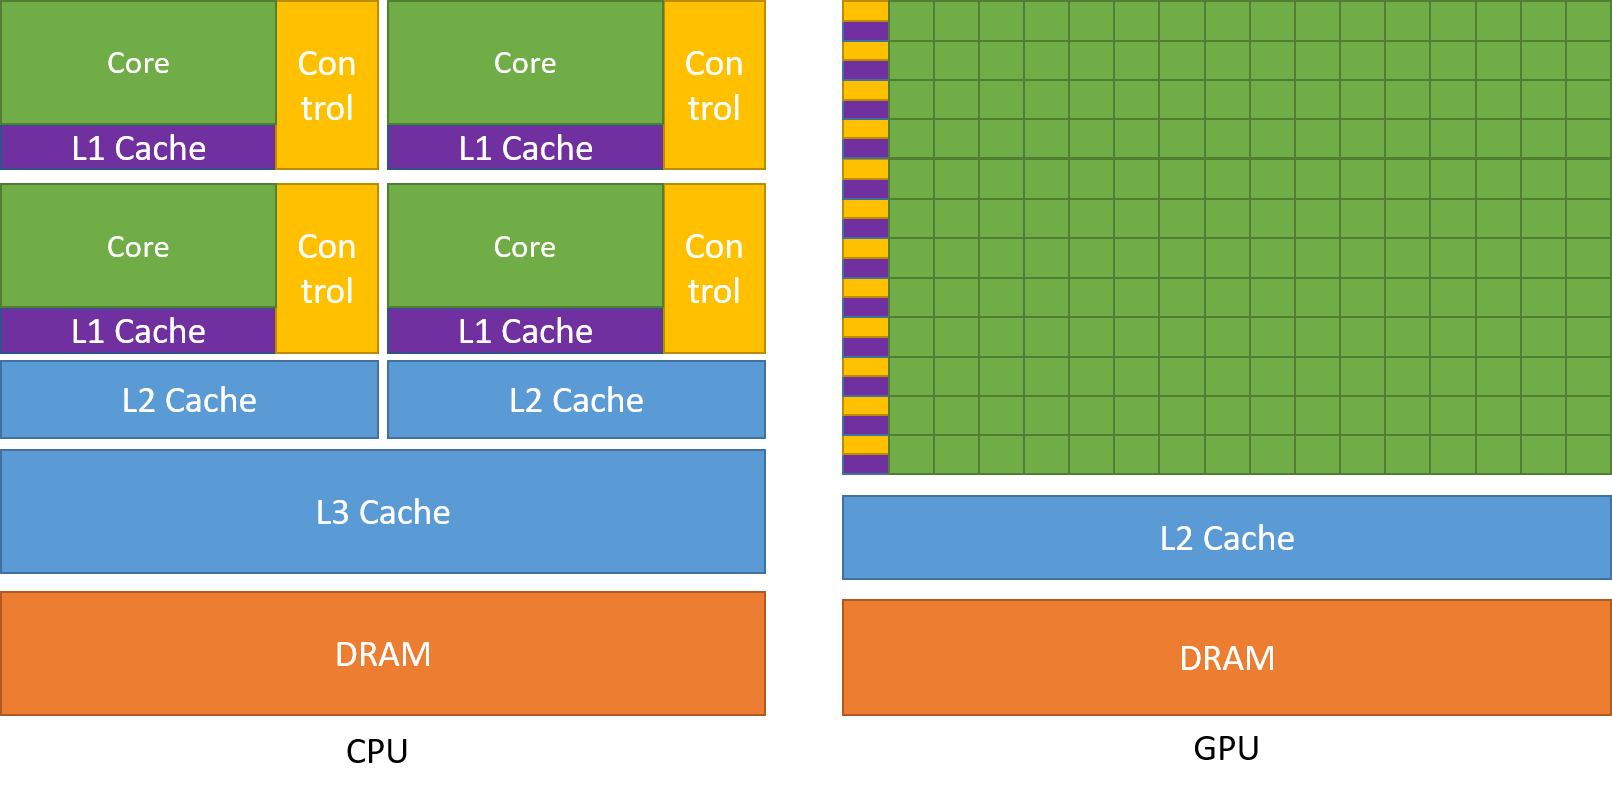
\includegraphics[width=0.65\linewidth]{Figures/gpu-devotes-more-transistors-to-data-processing.png}
	\caption{The GPU Devotes More Transistors to Data Processing}
	\label{fig:gpuvscpu}
\end{figure}

\subsection{CUDA Programming Model}
\label{sec:cudapromodel}
The CUDA parallel programming model addresses the challenges of scalable parallelism\cite{marccudaslides} while retaining 
accessibility for programmers familiar with languages such as C/C++. At the core of this model lie three 
fundamental abstractions—hierarchy of thread groups, shared memories, and barrier 
synchronization—introduced as minimal language extensions. These abstractions enable a combination of 
fine-grained and coarse-grained parallelism, directing programmers to partition problems into independently 
solvable sub-problems and fostering cooperative parallel problem-solving within thread blocks. 
This methodology not only maintains language expressivity but also permits automatic scalability, as each 
thread block can be scheduled on any accessible GPU multiprocessor, with the runtime system overseeing 
the physical multiprocessor count\cite{cuda2016best}. Figure~\ref{fig:cpuvsgpupro} shows an example of a CPU program vs a CUDA program.

\begin{figure}[htb]
    \centering
    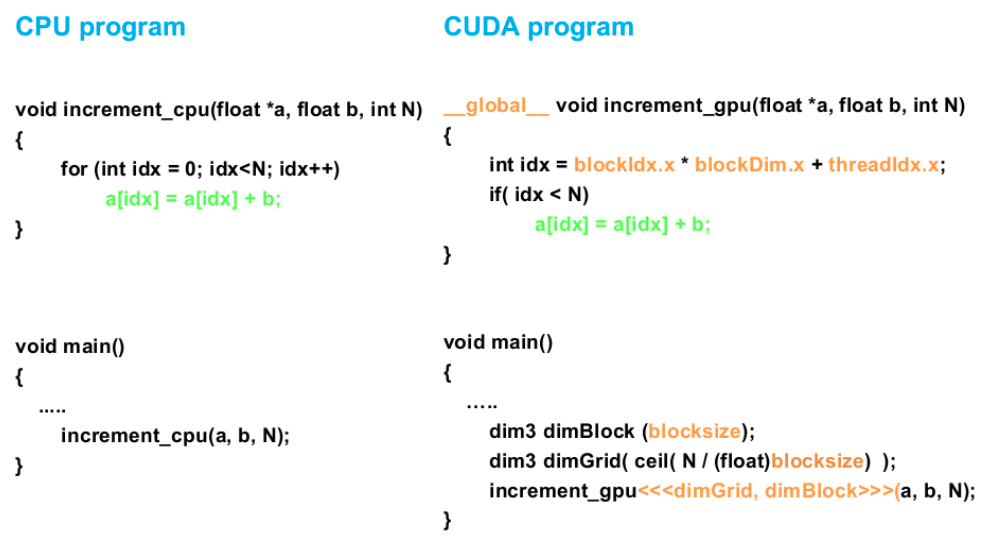
\includegraphics[width=0.85\linewidth]{Figures/CPUvsGPUprogram.png}
    \caption{Example of a CPU program vs a CUDA program}
    \label{fig:cpuvsgpupro}
\end{figure}

\subsubsection{Kernels}
\label{sec:kernels}
CUDA kernels are the fundamental building blocks of a CUDA program, representing the functions 
that execute on the GPU device (also referred to as the device) in parallel. In the context of 
CUDA, the CPU is referred to as the host, responsible for managing and orchestrating the execution 
of kernels on the device\cite{marccudaslides}. The device is typically composed of multiple streaming multiprocessors 
(SMs) that provide the parallel processing capability. A kernel is defined in the CUDA programming 
model using the \mintinline{cuda}{__global__} declaration specifier, which indicates that the function is callable 
from the host and executes on the device. The execution configuration of a kernel is specified 
using \mintinline{cuda}{<<<...>>>}, which determines the grid and block dimensions, 
thereby dictating the number of parallel threads and their organization during kernel execution\cite{cuda2016best}. 
This configuration allows programmers to efficiently utilize the available resources on the GPU 
and optimize the performance of their CUDA applications.

\subsubsection{Threads}
\label{sec:threads}
In the CUDA programming model, threads constitute the basic units of parallel execution and are 
organized within a hierarchical structure encompassing threads, thread blocks, and grids. Each 
thread is uniquely identified by its \mintinline{cuda}{threadIdx}, which is a multi-dimensional variable with up to 
three dimensions (x, y, and z)\cite{cuda2016best}. Thread limits are dictated by the GPU architecture, with the 
maximum number of threads per block typically capped at 1024. Threads are assembled into blocks, 
which are then organized into a grid. The \mintinline{cuda}{blockIdx} and \mintinline{cuda}{blockDim} variables identify the position 
of a specific block within the grid and the dimensions of each block, respectively. Thread and 
block dimensions can be one-, two-, or three-dimensional, offering flexibility in addressing the 
problem space in a manner that best accommodates the underlying data structure and computation. 
This hierarchical organization of threads and blocks enables efficient mapping of intricate, 
multi-dimensional problems onto the GPU's parallel processing resources, promoting optimal 
performance and resource utilization.

Thread blocks hold a pivotal role in the CUDA programming model\cite{marccudaslides}, functioning as a means to 
organize threads that collaboratively work on a specific sub-problem. Within a thread block, 
threads can communicate and synchronize their operations via shared memory, facilitating efficient 
data exchange and cooperative problem-solving. It is important to note that thread blocks can be 
executed in any order, both concurrently and sequentially, across the available SMs on a GPU. This 
flexibility permits automatic scalability, allowing the compiled CUDA program to adapt to varying 
GPU architectures and multiprocessor counts\cite{cuda2016best}. Consequently, thread blocks enable efficient utilization 
of GPU resources while ensuring that applications can scale effectively on diverse hardware configurations.

\subsubsection{Kernel Launch Parameters}
\label{sec:kernellaunchparameters}

When launching a CUDA kernel, the execution configuration specified plays a crucial role in determining 
the organization of threads and blocks for the kernel's execution on the GPU. The launch parameters 
within this syntax define the grid and block dimensions, which impact the performance and resource 
utilization of the application.

The launch parameters consist of two main components: the number of blocks per grid (\mintinline{cuda}{gridDim}) and the 
number of threads per block (\mintinline{cuda}{blockDim}). Both of these parameters can be specified as one-, two-, or 
three-dimensional structures, represented by dim3 variables in CUDA. The choice of dimensions depends 
on the problem space and the structure of the underlying data, with the aim of efficiently mapping the 
computation onto the GPU's resources.

For example, if a kernel is launched with the configuration \mintinline{cuda}{<<<gridDim, blockDim>>>}, it will create 
$gridDim.x * gridDim.y * gridDim.z$ blocks in the grid, with each block 
containing $blockDim.x * blockDim.y * blockDim.z$ threads. This results in a total of 
$(gridDim.x * gridDim.y * gridDim.z) * (blockDim.x * blockDim.y * blockDim.z)$ threads executing the 
kernel concurrently.

Selecting optimal launch parameters is essential for achieving maximum performance and resource 
utilization on the GPU\cite{cuda2019guide}. The choice of grid and block dimensions should consider factors such as the 
size of the problem, the hardware limitations of the GPU (e.g., maximum threads per block), and the 
level of parallelism required. Additionally, it is important to account for shared memory constraints, 
as larger block sizes may lead to increased shared memory requirements, potentially causing resource 
allocation issues or reduced parallelism\cite{cuda2019guide}.

By carefully choosing the launch parameters for a CUDA kernel, developers can create efficient, 
high-performance parallel applications that effectively exploit the capabilities of the underlying GPU hardware.\cite{cuda2019guide}

\subsection{CUDA by Example}
\label{sec:cudabyexample}

In the following section, we shall explore a fundamental example of CUDA programming by implementing a vector 
addition program. This hands-on approach will enable readers to gain a deeper understanding of the various components 
and concepts involved in writing and executing CUDA code. This example follows a GitHub repository, If you would like 
to explore this tutorial further and experiment with the code, it is available at the following \cite{Papatheodore2022}.

\definecolor{LightGray}{gray}{0.9}
\begin{minted}
[
frame=lines,
framesep=2mm,
baselinestretch=0.75,
bgcolor=LightGray,
fontsize=\footnotesize,
linenos,
samepage
]
{cuda}
#include <stdio.h>

// Size of array
#define N 1048576

// Kernel
__global__ void add_vectors(double *a, double *b, double *c)
{
	int id = blockDim.x * blockIdx.x + threadIdx.x;
	if(id < N) c[id] = a[id] + b[id];
}

// Main program
int main()
{
	// Number of bytes to allocate for N doubles
	size_t bytes = N*sizeof(double);

	// Allocate memory for arrays A, B, and C on host
	double *A = (double*)malloc(bytes);
	double *B = (double*)malloc(bytes);
	double *C = (double*)malloc(bytes);

	// Allocate memory for arrays d_A, d_B, and d_C on device
	double *d_A, *d_B, *d_C;
	cudaMalloc(&d_A, bytes);
	cudaMalloc(&d_B, bytes);
	cudaMalloc(&d_C, bytes);

	// Fill host arrays A and B
	for(int i=0; i<N; i++)
	{
		A[i] = 1.0;
		B[i] = 2.0;
	}

	// Copy data from host arrays A and B to device arrays d_A and d_B
	cudaMemcpy(d_A, A, bytes, cudaMemcpyHostToDevice);
	cudaMemcpy(d_B, B, bytes, cudaMemcpyHostToDevice);

	// Set execution configuration parameters
	//		thr_per_blk: number of CUDA threads per grid block
	//		blk_in_grid: number of blocks in grid
	int thr_per_blk = 256;
	int blk_in_grid = ceil( float(N) / thr_per_blk );

	// Launch kernel
	add_vectors<<< blk_in_grid, thr_per_blk >>>(d_A, d_B, d_C);

	// Copy data from device array d_C to host array C
	cudaMemcpy(C, d_C, bytes, cudaMemcpyDeviceToHost);

	// Free CPU memory
	free(A);
	free(B);
	free(C);

	// Free GPU memory
	cudaFree(d_A);
	cudaFree(d_B);
	cudaFree(d_C);

	return 0;
}
\end{minted}

\addvspace{5cm}

We initiate the process at line 17, where the memory requirement for an array comprising N double-precision elements is 
determined. Subsequently, memory allocation for vectors A, B, and C occurs on the host in lines 20-22. Continuing forward, 
lines 25-28 allocate memory on the device for the same vectors. It is worth noting the prevalent naming convention for device 
variables is ``d\_'' prefix to indicate device allocation.

The host input vectors A and B are copied to their device counterparts, d\_A and d\_B with \mintinline{cuda}{cudaMemcpy()} 
as seen in lines 38-39. To prepare for kernel 
launch, we set the kernel launch parameters in lines 44-45, defining the number of threads per block and the number of 
blocks per grid. The kernel is then launched in line 48, where the actual computation is executed.

Focusing on the \mintinline{cuda}{add_vectors} kernel function at line 7, a unique thread ID is identified in line 9 
for each thread within 
the grid. The \mintinline{cuda}{if} statement on line 10 serves to prevent memory access beyond the array's bounds, 
which may occur when 
the number of grid threads is not a multiple of the number of threads per block. For instance, if N has an extra element, 
\mintinline{cuda}{blk_in_grid} would equal 4097 due to the \mintinline{cuda}{ceil} function in line 45, resulting in a total of 
$4097*256 = 1048832$ threads. 
Without the \mintinline{cuda}{if} statement, the final thread would attempt to access memory beyond the array's boundaries.

In conclusion, the device output vector d\_C is copied to the host output vector C in line 51. Host memory is then freed 
in lines 54-56, followed by the release of device memory in lines 59-61.

\begin{figure}[htb]
    \centering
    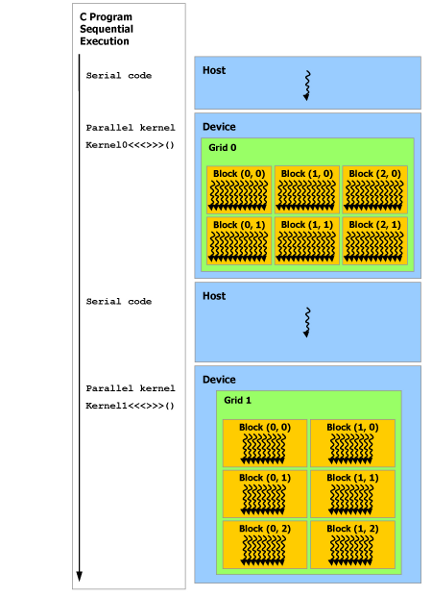
\includegraphics[width=0.65\linewidth]{Figures/heterogeneous-programming.png}
	\caption{Heterogeneous Programming Model for CUDA}
	\label{fig:heteropro}
\end{figure}

\subsection{CUDA Memory Model}
\label{sec:cudamemmodel}

\begin{figure}[htb]
    \centering
    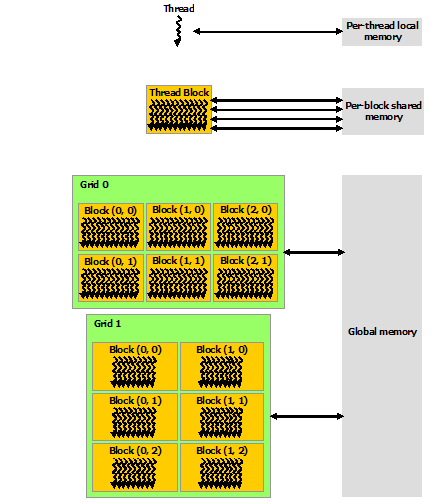
\includegraphics[width=0.65\linewidth]{Figures/memory-hierarchy.png}
	\caption{CUDA Memory Hierarchy}
	\label{fig:memhierarchy}
\end{figure}

The CUDA memory model is designed to accommodate the unique requirements of parallel programming 
on GPUs and consists of several distinct memory spaces. Host memory refers to the system memory 
allocated and managed by the CPU. In contrast, the GPU has its own memory spaces, including global, 
shared, and local memory\cite{cuda2016best}.

Global memory, accessible by all threads within a kernel as well as the host, serves as the primary 
means for data storage and communication between the host and the device. The lifetime of data in global 
memory spans from the point of allocation to deallocation, which is explicitly managed by the programmer. 
Although global memory offers a large storage capacity, it has higher access latency compared to other 
memory spaces on the GPU\cite{cuda2016best}.

Shared memory, as the name suggests, is a fast, on-chip memory space that can be shared among threads 
within the same thread block. This memory space enables efficient inter-thread communication and data 
exchange, making it particularly useful for problems that require threads to cooperate and share 
information while solving sub-problems. However, shared memory is limited in capacity, and its contents 
are only available for the duration of a thread block's execution\cite{cuda2016best}.

Local memory is private to each individual thread and is used for storing thread-specific data, such as 
function call frames and automatic variables. While local memory is accessible only by the thread that 
owns it, it allows threads to store temporary data without affecting other threads. Similar to global memory, 
local memory resides off-chip, and therefore, its access latency is higher than that of shared memory.

Refer to Figure~\ref{fig:memhierarchy} for a visual representation of the CUDA memory hierarchy.

\subsection{GPU Microarchitecture}
\label{sec:gpumicroarchitecture}

We introduce the fundamental concepts of GPU microarchitecture, highlighting their 
relation to the CUDA programming model\cite{cuda2016best}. Understanding these core principles allows for a deeper 
comprehension of the efficient execution of parallel workloads on GPUs and informs the development 
of effective CUDA applications.

\subsubsection{SIMT and SIMD}
\label{sec:simdandsimt}

SIMT (Single Instruction, Multiple Thread) and SIMD (Single Instruction, Multiple Data) 
constitute vital parallel execution models that impact the performance of GPU architectures
and their integration with the CUDA programming model. SIMT operates by executing identical 
instructions on distinct threads, while SIMD conducts the same operation on multiple data elements. 
NVIDIA GPUs utilize the SIMT paradigm, permitting threads to be organized into warps that 
execute instructions concurrently, thus optimizing resource usage and reducing thread management 
overhead\cite{cuda2016best}. The CUDA programming model corresponds directly to the SIMT architecture, empowering developers 
to harness the inherent parallelism of GPUs while efficiently handling threads, memory, and 
synchronization to achieve exceptional parallel computing performance.

\subsubsection{Streaming Multiprocessors (SMs)}
\label{sec:sm}

Streaming Multiprocessors (SMs) are the primary building blocks of NVIDIA GPUs, acting as the core 
computational units that enable efficient parallel processing. Each SM houses multiple execution 
units, registers, and shared memory, facilitating the concurrent execution of a large number of threads. 
In CUDA, developers organize threads into blocks, which are then scheduled onto SMs\cite{cuda2016best}. This arrangement 
allows for effective management of thread parallelism, memory, and synchronization, ensuring optimal GPU 
resource utilization and high-performance parallel computing.

\subsubsection{Warp and Warp Scheduling}
\label{sec:warp}

Warps and warp scheduling are essential components of GPU architectures, particularly in the context 
of CUDA programming. In CUDA, a warp is a group of threads, typically 32, that execute simultaneously 
on a single streaming multiprocessor (SM). Threads within a warp share a common program counter and 
follow a simultaneous execution pattern, optimizing resource utilization and reducing thread management 
overhead. Warp scheduling, on the other hand, is instrumental in managing how warps execute on SMs. 
Different GPU architectures use various scheduling policies, determining the selection and instruction 
issuance for ready warps\cite{cuda2016best}. Efficient warp scheduling is crucial for maximizing GPU resource utilization 
and overall performance.


\section{MWP-CWP}
\label{sec:mwp-cwp}

The MWP-CWP analytical model offers a novel approach to understanding the performance of GPU 
architectures by examining the parallelism exhibited by MWP and CWP. As multithreaded architectures, GPUs allow multiple warps 
to be executed concurrently on a streaming multiprocessor (SM), effectively hiding the execution 
costs of these warps. The MWP-CWP model focuses on determining the maximum number of warps that 
can access memory simultaneously and the number of warps that an SM processor can execute during 
a memory warp waiting period. By carefully analyzing the relationship between MWP and CWP, this 
model provides valuable insights into the factors that govern execution time, revealing whether 
it is dominated by computation or memory access costs. Through a series of illustrative cases, we 
will demonstrate the importance of sufficient warps and the intricate interplay between MWP and CWP 
in optimizing GPU performance.\cite{DBLP:conf/isca/HongK09,marcmwpcwpslides}

\begin{figure}[H]
	\centering % <-- added
	\begin{subfigure}[b]{0.55\textwidth}
        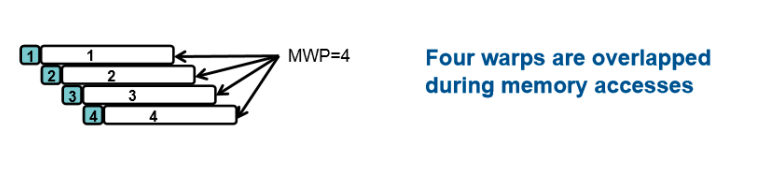
\includegraphics[width=\linewidth]{Figures/MWP.png}
        \caption{MWP}
        \label{fig:mwp}
	\end{subfigure}\hfil % <-- added
	\begin{subfigure}[b]{0.45\textwidth}
		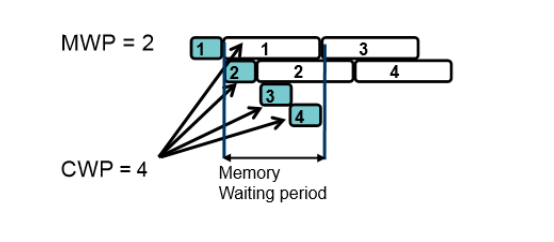
\includegraphics[width=\linewidth]{Figures/CWP.png}
	    \caption{CWP}
	    \label{fig:cwp}
	\end{subfigure}
	\label{fig:mwpcwpmodel}
    \caption{MWP-CWP model}
\end{figure}

\subsection{$MWP \leq CWP$}
\label{sec:mwp-cwp:1}

In the case where CWP is greater than MWP, the application's performance exhibits a distinct 
characteristic: computation cycles are effectively hidden by memory waiting periods. This implies 
that the computational resources are kept busy while the memory accesses are being processed, 
leading to a more efficient use of the available resources. However, the overall performance of 
the application is dominated by the memory cycles, as the computational work is executed in parallel 
with memory access operations. In other words, the system exhibits a higher degree of parallelism in 
computation than in-memory operations. This implies that while the application effectively utilizes 
the available computational resources, it may face limitations in leveraging memory-level parallelism. 
This imbalance between CWP and MWP can result in the underutilization of memory bandwidth and potentially 
lead to performance bottlenecks.\cite{DBLP:conf/isca/HongK09,marcmwpcwpslides}

\begin{figure}[htb]
    \centering
    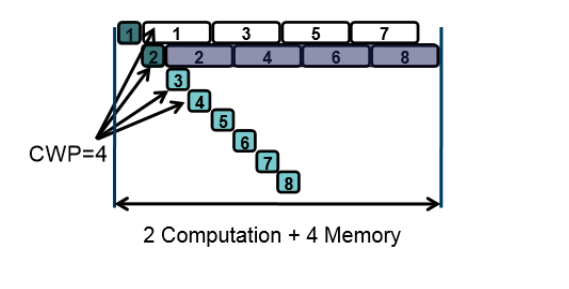
\includegraphics[width=0.65\linewidth]{Figures/cwpgreaterthanmwp.png}
	\caption{Computation cycles are concealed by memory waiting periods, 
             resulting in the overall performance being predominantly dictated by memory cycles.}
	\label{fig:cwpgreaterthanmwp}
\end{figure}

\subsection{$MWP > CWP$}
\label{sec:mwp-cwp:2}

In the scenario where MWP is greater than CWP, the application's performance demonstrates a contrasting behavior: 
memory accesses are predominantly hidden due to the high MWP. This means that the memory subsystem is capable 
of handling multiple memory requests concurrently while the computation resources are being utilized, 
effectively masking memory latencies. As a result, the overall performance of the application is dominated 
by the computation cycles, since the memory accesses are efficiently processed in parallel with the computational 
work. To put it differently, the application's performance may be hindered due to an imbalance between memory 
and computational resources. This disparity indicates that the application has a higher degree of parallelism 
in memory access than in computation, which can potentially result in the underutilization of computational 
resources.\cite{DBLP:conf/isca/HongK09,marcmwpcwpslides}

\begin{figure}[htb]
    \centering
    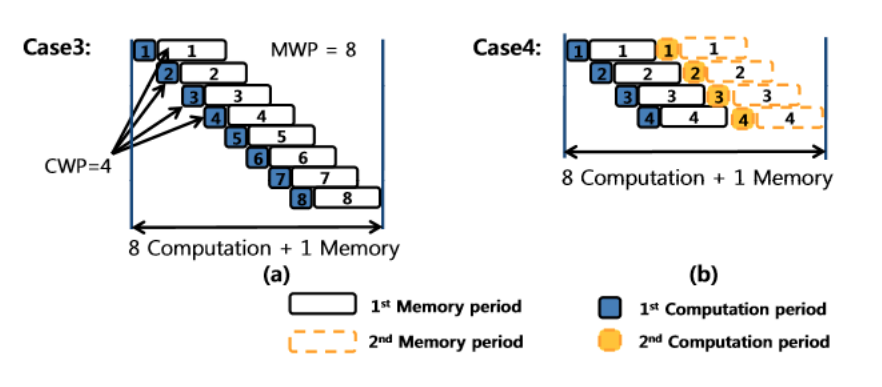
\includegraphics[width=0.65\linewidth]{Figures/mwpgreaterthancwp.png}
	\caption{Memory accesses are largely concealed by high MWP, 
            leading to the overall performance being primarily governed by computation cycles.}
	\label{fig:mwpgreaterthancwp}
\end{figure}




 
\chapter{Theoretical Foundations}
\label{ch:foundations}



Let ${\cal P}$ be a multithreaded program to be executed on a specific 
multiprocessor.
Parameters influencing  the performance of ${\cal P}$ include: 
\begin{inparaenum}[(i)]
\item {\em data parameters}, specifying the size and possibly
  structural characteristics of the data, 
\item {\em hardware parameters}, specifying
  characteristics of hardware resources, and
\item {\em program parameters}, specifying
how   work (e.g. threads) is mapped to
  hardware resources.
\end{inparaenum}
%% 	
By fixing the target architecture, the hardware parameters, say, ${\bm
  H} = \left(H_1, \ldots, H_h\right)$ become fixed and we can assume
that the performance of ${\cal P}$ depends only on data parameters
${\bm D} = \left(D_1, \ldots, D_d\right)$ and program parameters ${\bm
  P} = \left(P_1, \ldots, P_p\right)$.
%%
\ifoldversion Moreover, an optimal choice of ${\bm P}$ naturally
depends on a specific choice of ${\bm D}$.  \fi
%%
For example, in programs targeting GPUs 
%(e.g. programs written in {\cuda}),   %\ or OpenCL programs
the parameters ${\bm D}$ are typically dimension sizes of data
structures, like arrays, while ${\bm P}$ typically specifies the
format of the grid and the format of the thread blocks.
%(see Section~\ref{sec:embodiment} for further details of 
%this technique applied to \cuda).
%%


Let ${\cal E}$ be a high-level performance metric (running time, memory consumption)
for ${\cal P}$ that we want to
optimize.  More precisely, given the values of the data parameters
${\bm D}$,  our goal is to find values of the program parameters
${\bm P}$ such that the execution of ${\cal P}$ optimizes
${\cal E}$.  
%\toremove{Here, optimizing could mean maximizing, as in the case of a
%performance metric such as hardware occupancy, or minimizing, as in the case
%of a performance metric like execution time. }
Performance prediction models attempt to estimate ${\cal E}$ from a
combination of ${\bm P}$, ${\bm D}$, ${\bm H}$, and some model- or
platform-specific low-level metrics ${\bm L} = (L_1, \ldots,
L_\ell)$ (memory bandwidth, cache miss rate, etc.).
It is natural to assume that these low-level performance
metrics are themselves functions of ${\bm P}$, ${\bm D}$, ${\bm
  H}$.  This is an obvious observation from models based on PRAM such
as TMM~\cite{DBLP:journals/fgcs/MaAC14} and
MCM~\cite{DBLP:conf/parco/HaqueMX15}.
%%

Therefore, we look to obtain values for these low- and high-level metrics
given values for program, and data parameters.
To address our optimization goal, we  use the following strategy.
At the compile-time of program ${\cal P}$,  for each metric, 
we determine a mathematical formula expressing that metric as a  
function of the data and program parameters.
This mathematical formula takes the 
form of what we call a {\em rational program}.
%with some selected values of $D_1, \ldots, D_d$ which do not need to be the ones that  ${\cal P}$ will be executed on.
At the runtime of ${\cal P}$, given specific values of ${\bm D}$
and a choice of ${\bm P}$, we can evaluate the rational program to
obtain a value for each metric and thus for ${\cal E}$.  Repeating
this for all possible choices of ${\bm P}$ (assumed to be finite
in number) yields values of ${\bm P}$
optimizing ${\cal E}$.  This strategy is detailed in
Section~\ref{sec:steps}, while Section~\ref{sect:ratprog} 
is dedicated to the notion of a rational program.

One could view a rational program as a computer program that,
for input values $x_1, \ldots, x_n$, computes and returns a value
$y = f(x_1, \ldots, x_n)$, where $f$ is a function in the sense of a
programming language, say C/C++.  However, a rational program is 
more than that, due to the process we use to determine $f$.

%% Specifically, the encoding of some model as a flow chart 
%% whose nodes can then be approximated as a rational function
%% is a powerful idea which can be used
%% to simplify models and extrapolate results.

%We  take the remainder of this section to describe the 
%ideas underpinning rational programs.

\section{Rational Programs}
\label{sect:ratprog}

Let $X_1, \ldots, X_n, Y$ be pairwise different
variables\footnote{Variables refer to both its mathematical meaning
  and programming language concept.}.  Let ${\cal S}$ be a sequence of
three-address code (TAC~\cite{Aho:1986:CPT:6448}) instructions such
that the variables occurring in ${\cal S}$ that are never
assigned a value by an instruction
of ${\cal S}$ are exactly $X_1, \ldots, X_n$.


\begin{definition}
\label{defi:rationalprogram}
We say that the sequence ${\cal S}$ is a
{\em rational program} in $X_1, \ldots, X_n$ evaluating $Y$
if the following two conditions hold:
\begin{enumerateshort}
\item every arithmetic operation used in ${\cal S}$ is either an addition,
  a subtraction, a multiplication, a division, 
  or a comparison (for equality or the natural order $\le$)
  %($=$, $<$),
  of two rational numbers numbers, in either fixed or arbitrary precision.
\item after specializing in ${\cal S}$ the variables $X_1, \ldots, X_n$ to
      rational numbers $x_1, \ldots, x_n$, the execution of the 
      specialized sequence always terminates and the last
      executed instruction assigns a rational number to $Y$.
\end{enumerateshort}
\end{definition}

It is worth noting that the above 
definition can easily be extended to include
Euclidean division, the integer part operations floor and ceiling,
and arithmetic over rational numbers.
For Euclidean division one can write a rational program
evaluating the quotient $q$ of integer $a$ by $b$, 
leaving the remainder $r$ to be simply calculated as $a - qb$.
Then, floor and ceiling can be computed via Euclidean division.
Rational numbers and their associated arithmetic are easily implemented using
only integer arithmetic.
Therefore, by adding these operations to 
Definition~\ref{defi:rationalprogram}, the 
class of rational programs does not change.
We regard rational programs as such henceforth.
%Thus, we add such operations to the definition
%of a rational program and adopt this definition henceforth.

\section{Rational Programs as Flowcharts}

For any sequence ${\cal S}$ of computer program 
instructions, one can associate  ${\cal S}$
with a {\em control flow graph} (CFG).
In the CFG of ${\cal S}$, the nodes are the {\em basic blocks} of ${\cal S}$.
\iffalse 
the sub-sequences of ${\cal S}$ such that 
\begin{enumerate}[(i)]
	\item  each instruction except the last one is not a branch, and
	\item which are maximum in length with property (i).
\end{enumerate}
Moreover, in the CFG of ${\cal S}$, 
there is a directed edge from a basic block $B_1$ to a basic block
$B_2$ whenever, during the execution of ${\cal S}$, one can jump from
the last instruction of $B_1$ to the first instruction of $B_2$.
%%
\fi
Recall that  a {\em flowchart} is another
graphic representation of a sequence of computer program  instructions.
In fact, CFGs can be seen as particular flowcharts.
%%

If, in a given flowchart ${\cal C}$, every arithmetic
operation occurring in every (process or decision) node is
either an addition, subtraction, multiplication, or comparison of integers
in either fixed or arbitrary precision
then ${\cal C}$ is the flowchart of a rational sequence of computer
program instructions.
Therefore, it is meaningful to depict rational programs
using flowcharts, and vice versa, 
flowcharts as rational programs.
For example, one could consider the metric 
of theoretical {\em hardware occupancy} as defined by 
NVIDIA. 
The following example details its definition, 
its depiction as a flowchart, and its dependency on
program, data, and hardware parameters.

\begin{example}
\label{ex:cuda}
{\em
The hardware {\em occupancy} is a measure of a program's effectiveness in using
the Streaming Multiprocessors (SMs) of a GPU.
It is calculated from a number of hardware parameters, namely:
\begin{itemizeshort}
\item[-] the maximum number $R_{\rm max}$ of registers per thread block,
\item[-] the maximum number $Z_{\rm max}$ of shared memory words per thread block,
\item[-] the maximum number $T_{\rm max}$ of threads per thread block,
\item[-] the maximum number $B_{\rm max}$ of thread blocks per SM and 
\item[-] the maximum number $W_{\rm max}$ of warps per SM,
\end{itemizeshort}
as well as low-level kernel-dependent performance metrics, namely:
\begin{itemizeshort}
\item[-] the number $R$ of registers used per thread and 
\item[-] the number $Z$ of shared memory words used per thread block,
\end{itemizeshort}
and a program parameter, namely the 
number $T$ of threads per thread block.
%%
The occupancy of a {\cuda} kernel is defined as
the ratio between the number of active warps
per SM and the maximum number of warps per SM, namely:
\begin{equation}
\label{eq:occupancy}
W_{\rm active} / W_{\rm max}, \ \ {\rm where} \ \ 
    W_{\rm active} \fixed{\leq}{Changed to an inequality to highlight the
    upper bound given by this equation: Fine.} \min \left( \lfloor B_{\rm active} T / 32 \rfloor, W_{\rm max}  \right)
\end{equation}
and $B_{\rm active}$ is given by the flowchart
in Figure~\ref{fig:occupancysimpleflowchart}.
%%
This flowchart shows
how one can derive a rational program computing
$B_{\rm active}$ from $R_{\rm max}$, $Z_{\rm max}$,
$T_{\rm max}$, $B_{\rm max}$, $W_{\rm max}$, $R$, $Z$, $T$.
%%
It follows from Formula (\ref{eq:occupancy})
that $W_{\rm active}$ can also be computed 
by a rational program from $R_{\rm max}$, $Z_{\rm max}$,
$T_{\rm max}$, $B_{\rm max}$, $W_{\rm max}$, $R$, $Z$, $T$.
%%
Finally, the same is true for the occupancy of a {\cuda} kernel
using $W_{\rm active}$ and $W_{\rm max}$.
}
\end{example}
\tikzset{%
	>={Latex[width=2mm,length=2mm]},
	% Specifications for style of nodes:
	base/.style = {rectangle, rounded corners, draw=black,
		minimum width=4cm, minimum height=1cm,
		text centered, font=\sffamily},
	activityStarts/.style = {base, fill=blue!30},
	startstop/.style = {base, fill=red!30},
	activityRuns/.style = {base, fill=green!30},
	process/.style = {base, minimum width=2.5cm, fill=blue!15,
		font=\ttfamily},
	ifstatement/.style = {base, diamond, aspect=2.5, scale=0.7, font=\Large},
}
\usetikzlibrary{shapes.geometric}
\begin{figure}
	\centering
\begin{tikzpicture}[node distance=2.5cm,scale=.5, 
    every node/.style={fill=white,scale=.7, font=\sffamily}, align=center]
  % Specification of nodes (position, etc.)
  
  \node (activemax) [ifstatement] {$T \, B_{max} \leq 32 \, W_{max}$ and\\ $R \,  T \,  B_{\rm max} \leq R_{\rm max}$ and\\ $Z \,  B_{\rm max} \leq Z_{\rm max}$?};
  
  \node (activewmax) [ifstatement, below of=activemax, yshift=-9.5em] {$32 \,  W_{\rm max} \leq T \,  B_{\rm max}$, and\\ $32 \,  W_{\rm max} \,  R \leq R_{\rm max}$ and\\ $32 \,  W_{\rm max} \,  Z \leq Z_{\rm max} \,  T$?};
  
  \node (activermax) [ifstatement, below of=activewmax, yshift=-9.5em] {$R_{\rm max} \leq R \,  T \,  B_{\rm max}$ and\\ $R_{\rm max} \leq R \,  32 \,  W_{\rm max}$ and\\ $R_{\rm max} \,  Z \leq R \,  T \,  Z_{\rm max}$?};

  \node (activezmax) [ifstatement, below of=activermax, yshift=-9.5em] {$Z_{\rm max} \leq B_{\rm max} \,  Z$ and\\ $Z_{\rm max} \,  T \leq 32 \,  W_{\rm max} \,  Z$ and\\ $Z_{\rm max} \,  R \,  T \leq Z \,  R_{\rm max}$?};

  \node (bmax) [process, right of=activemax, xshift=16em, text width=12em] {$B_{active} = B_{max}$};
  \node (wmax) [process, right of=activewmax, xshift=16em, text width=12em] {$B_{\rm active} =  \lfloor( 32 \,  W_{\rm max})/T  \rfloor$};
  \node (rmax) [process, right of=activermax, xshift=16em, text width=12em] {$B_{\rm active} =  \lfloor( R_{\rm max}/(R \,  T) \rfloor$};
  \node (zmax) [process, right of=activezmax, xshift=16em, text width=12em] {$B_{\rm active} =  \lfloor Z_{\rm max}/Z \rfloor$};
      
  \node (fail) [startstop, below of=activezmax, yshift=-3.5em] {$B_{\rm active} = 0$
(Failure to Launch)};

  \draw[->] (activemax) -- node[] [yshift=0.45em]{No} (activewmax);
  \draw[->] (activewmax) -- node[] [yshift=0.45em]{No} (activermax);
  \draw[->] (activermax) -- node[] [yshift=0.45em]{No} (activezmax);
  \draw[->] (activezmax) -- node[] [yshift=0.45em]{No} (fail);  
  
  \draw[->] (activemax) -- node[] [xshift=-0.5em]{Yes} (bmax);
  \draw[->] (activewmax) -- node[] [xshift=-0.5em]{Yes} (wmax);
  \draw[->] (activermax) -- node[] [xshift=-0.5em]{Yes} (rmax);
  \draw[->] (activezmax) -- node[] [xshift=-0.5em]{Yes} (zmax);
  
  \draw[->]  ([shift=({0,2.5em})]activemax.north) to (activemax.north);
\end{tikzpicture}
\caption{Rational program (presented as a flow chart) for 
the calculation of the number of active blocks per streaming processor
in a {\cuda} kernel.}
\label{fig:occupancysimpleflowchart}
\end{figure}




\section{Piece-Wise Rational Functions in Rational Programs}
\label{sec:prf_rp}

We begin with an observation describing the fact that a rational program
can be viewed as a piece-wise rational function \footnote{Here, rational function is in the
	sense of algebra, see Section~\ref{sec:paramest}.} .
\begin{observation}
\label{obs:rationality}
{\em
Let ${\cal S}$ be a rational program in $X_1, \ldots, X_n$ evaluating $Y$.
%%
Let $s$ be any instruction of ${\cal S}$ other than a branch or an
integer part instruction.  
Hence, this instruction can be of the form
$C = A + B$, $C = A - B$, $C = A \times B$, where $A$ and
$B$ can be any rational number.
%
Let $V_1, \ldots, V_v$ be the variables that are defined
at the entry point of the basic block of the instruction $s$.
An elementary proof by induction yields the following fact.
There exists a rational function in $V_1,
\ldots, V_v$ denoted $f_s(V_1, \ldots, V_v)$
such that $C = f_s(V_1, \ldots, V_v)$ for all possible values of
$V_1, \ldots, V_v$.
%
From there, one derives the following observation.
There exists a partition ${\cal T} = \{ T_1, T_2, \ldots    \}$ 
of ${\Q}^n$ (where ${\Q}$ denotes the field of rational numbers)
and rational functions $f_1(X_1, \ldots, X_n)$, 
$f_2(X_1, \ldots, X_n)$, $\ldots\ $
such that, if $X_1, \ldots, X_n$ receive respectively 
the values $x_1, \ldots, x_n$, then
the value of $Y$ returned by ${\cal S}$ is one of
$f_i(x_1, \ldots, x_n)$ such that
$(x_1, \ldots, x_n) \in T_i$ holds.
%%
In other words, ${\cal S}$ computes $Y$ as a
{\em piece-wise rational function} \, (PRF).
Notice if ${\cal S}$ contains
only one basic block then ${\cal S}$ 
can be trivially given by a single rational function.

Example~\ref{ex:cuda} 
shows that the hardware occupancy of a {\cuda}
kernel is given as a piece-wise rational function
in the variables $R_{\rm max}$, $Z_{\rm max}$,
$T_{\rm max}$, $B_{\rm max}$, $W_{\rm max}$, $R$, $Z$, $T$.
Hence, in this example, we have $n = 8$, 
and, as shown by Figure~\ref{fig:occupancysimpleflowchart}, 
its partition of ${\Q}^n$ contains 5 parts
as there are 5 terminating nodes in the flowchart.

}
\end{observation}

Suppose that a flowchart ${\cal C}$ 
representing the rational program ${\cal R}$
is partially known; to be precise, suppose that the decision nodes
are known (that is, the mathematical expressions
defining them are known) while the process nodes
are not. 
Then, from Observation~\ref{obs:rationality},
each process node can be given by
a one or more rational functions.
Trivially, a single formula can also
be seen as a flowchart with a single process node.
Determining each of those rational functions
can be achieved by solving an \textit{interpolation}
or \textit{curve fitting} problem.
More generally, if the sequence of instructions in 
a process node involves non-rational functions (e.g. $\log$)
we can apply Stone-Weierstrass Theorem~\cite{stone1948generalized}
to approximate each of those by a PRF.


It then follows that any performance metric,
which can be depicted as a flow chart
or a formula,
can also be represented as a piece-wise rational function, 
and thus a rational program. 
For high-level performance metrics, which relies on low-level metrics,
one could work recursively, first determining rational programs
for the low-level metrics which depend on $\bm{P}$, $\bm{D}$, and $\bm{H}$,
and then constructing a rational program for the high-level metric 
from those rational programs.
Hence, by this recursive construction, we can fully
determine a rational program for 
a high-level metric depending only on $\bm{P}$, $\bm{D}$, and $\bm{H}$.
\fixed{Of course, hardware parameters could be fixed given a target architecture
to yield a rational program which depends only on $\bm{P}$ and $\bm{D}$.}{ And then what?}
\fixed{Again, notice that even where formulas for low-level metrics are not known,
it is still possible to estimate them as PRFs, and thus rational programs,
via a curve fitting.}{Haven't we said that already. Yes, but I believe this is repetition 
is for emphasis that maybe some readers may miss when skimming through a "theory" section.}


As an example, consider occupancy (Example~\ref{ex:cuda}).
One could first determine PRFs for the number of
registers user per thread and the amount of shared memory
used per thread block. Then, a PRF is determined
for the number of active blocks (Figure~\ref{fig:occupancysimpleflowchart})
from these two low-level metrics, and a few more hardware
and program parameters. 
Thus, by recursive construction, 
we have a PRF depending only on 
program and hardware parameters.

%Recall that building such a rational
%program ${\cal R}$ is our goal.
%Once ${\cal R}$ is known, it can be
%used at runtime (that is, when the program ${\cal P}$ is run
%on specific input data) to compute optimal values for the program
%parameters. This is exactly what is achieved in our tool
%implementing this technique. 
%Before exploring this tool
Lastly, we make one final remark. 
We assumed that the decision nodes in the flowchart of the rational program were known, 
however, we could relax this assumption.
Indeed, each decision node is given by
a series of rational functions.
Hence, those could also be determined by
solving curve fitting problems.
However, we do not discuss this further
since it is not needed in our proposed
technique or implementation presented in the remainder of this thesis.

\chapter{An Overview of KLARAPTOR}
\label{ch:overview}

In this chapter, we present an overview of KLARAPTOR, a compile-time tool designed to optimize the performance of 
CUDA kernels by dynamically choosing the most suitable thread block configuration. We discuss the underlying theory 
of rational programs and the MWP-CWP performance model, which form the basis of KLARAPTOR's functionality. Furthermore, 
we explain the process of building and utilizing rational programs to determine optimal kernel launch parameters, 
detailing both the compile-time and runtime aspects of the tool. This chapter aims to provide an in-depth understanding of 
KLARAPTOR's methodology and how it contributes to enhancing kernel performance in CUDA applications.

\section{Dynamic Optimization of CUDA Kernel Launch Parameters}
\label{sec:klaraptor}

%\begin{figure*}[ht]
%	\centering
%	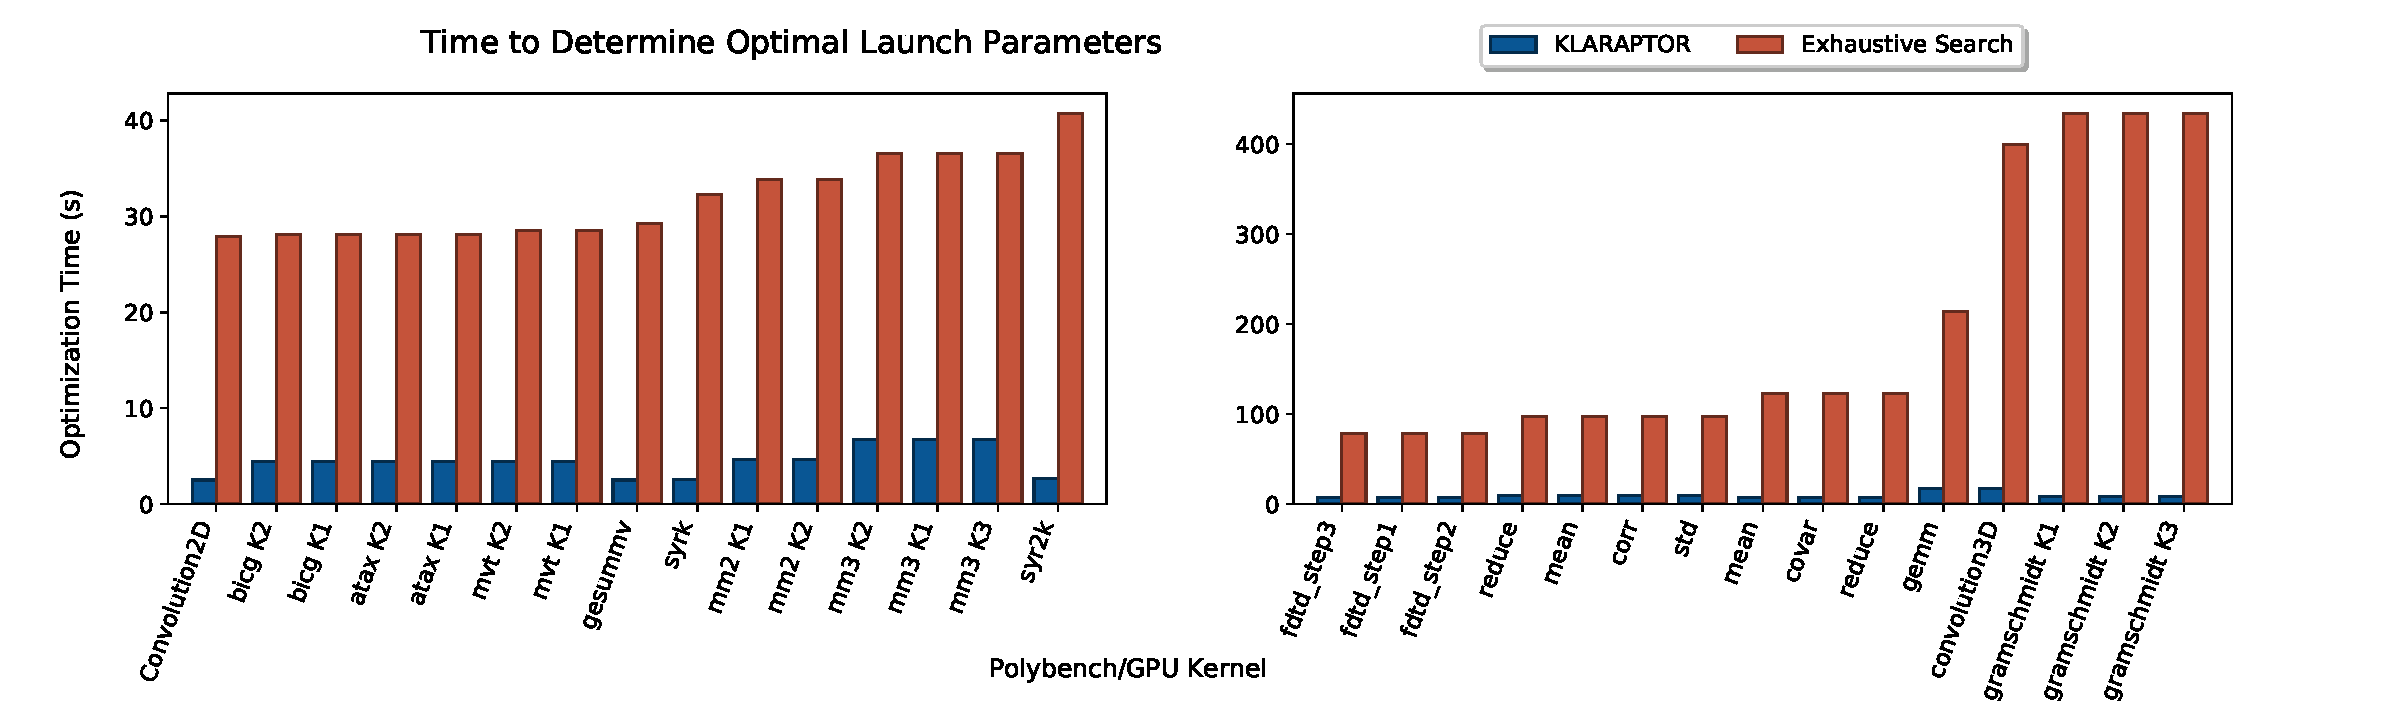
\includegraphics[width=\textwidth,clip,trim={1.5em, 1em, 5.5em, 1.2em}]{Figures/SystemTimesAll.pdf}
%	\caption{Comparing cumulative times to determine optimal launch parameters for data sizes $32 \leq N \leq 2048$ for each kernel in \texttt{Polybench/GPU}.}\label{fig:systemtimesall}
%\end{figure*}

The theory of rational programs is put into practice for the {\cuda}
programming model by our tool KLARAPTOR.  KLARAPTOR is a compile-time
tool implemented using the LLVM Pass Framework and the {\mwpcwp}
performance model to dynamically choose a {\cuda} kernel's launch
parameters (thread block configuration) which optimize its
performance.  Most high-performance computing applications require
computations be as fast as possible and so kernel performance is
simply measured as its execution time.

As mentioned in Chapter~\ref{ch:intro}, 
thread block configurations drastically affect the running time of a kernel.
Determining optimal thread block configurations typically follows some heuristics, for example, 
constraining block size to be a multiple of 32 \cite{cuda2016best}. However, it is known
that the dimension sizes of a thread block, not only its total size, affect performance~\cite{DBLP:journals/tjs/TorresGL13,DBLP:conf/cascon/ChenCKMX15}.
Moreover, since thread block configurations are intimately tied to the size of data being operated on,
it is very unlikely that a static thread block configuration optimizes the performance 
of all data sizes. Our tool effectively uses rational programs to 
dynamically determine the thread block configuration 
which minimizes the execution time of a particular 
kernel invocation, considering
the invocation's particular data size 
and target architecture. 
This is achieved in two main steps. 
\begin{enumerate}
	\item At the compile-time of a {\cuda} program, its kernels are analyzed in order to
	build rational programs estimating some performance metrics for each individual kernel.
	Each rational program, written as code in the C language,
	is inserted into the code of the {\cuda} program
	so that it is called before the execution of the corresponding kernel.
	\item At runtime, immediately preceding the launch of a kernel, where data parameters have specific values, the rational program is evaluated to 
	determine the thread block configuration which optimizes the performance of the kernel. The kernel
	is then launched using this thread block configuration. 
\end{enumerate} 

Not only are we concerned with kernel performance, but also
programmer performance. By that, 
we mean the efficiency of a programmer to produce 
optimal code. When a programmer is attempting to optimize a kernel, choosing optimal launch
parameters can either be completely ignored, 
performed heuristically, determined by trial and error, or determined by an exhaustive search.
The latter two options quickly become infeasible as data sizes grow large.
Regardless, any choice of optimal thread block configuration is likely to optimize
only a single data size. 

For KLARAPTOR to be practical, not only does the choice of optimal
kernel launch parameters need to be correct, but it must also
be more efficient than trial and error or exhaustive search.
Namely, the compile-time analysis cannot add too much 
overhead to the the compilation time and the
runtime decision of the kernel launch parameters cannot
overwhelm the program execution time. 
For the former, our analysis is performed
quickly by analyzing kernel performance on only small data sizes, 
and then results are extrapolated.
For the later, the rational program evaluation is quick and simple, 
being only the evaluation of a few rational functions.
Moreover, we maintain a runtime invocation history
to instantly provide results for future kernel launches.
Our implementation is detailed in Chapter~\ref{ch:implementation}.
%In the remainder of this section we highlight the performance of
%KLARAPTOR.

We have made use of the \texttt{Polybench/GPU}
benchmark suite as an empirical
evaluation of the correctness of our tool on a range of {\cuda} programs.
In Figure~\ref{fig:kernelperfintro} we have already seen that KLARAPTOR
accurately predicts the optimal or near-optimal thread block
configuration. 
Before presenting more detailed results and 
experimentation in Chapter~\ref{ch:performance},
we describe the steps followed by our tool
to build and use rational programs for 
determining a thread block configuration which optimizes
performance.

%Let us begin with kernel performance. 
%Other optimization techniques (see Section~\ref{sec:relatedworks})
%focus on improving the performance of a kernel by code optimizations. Our techniques
%rather focuses on simply modifying program parameters for performance. 
%focus on auto-tuning, static source code analysis, or machine learning applied to over-simplified 
%models.


\section{An Algorithm to Select Program Parameters}
\label{sec:steps}

In this section the notations and hypotheses are the same as in
Chapter~\ref{ch:foundations}.
Namely, ${\cal E}$ is a high-level performance metric for the 
multithreaded program ${\cal P}$, 
${\bm L}$ is a set of low-level metrics of size $\ell$,
and ${\bm P}$, ${\bm D}$, ${\bm H}$ are
sets of program, data, and hardware parameters, respectively. 
Recall ${\bm P}$ has size $p$.
%%
Let us assume that the values of ${\bm H}$ are known at the compile-time of ${\cal P}$
while the values of ${\bm D}$ are known at runtime.
Further, let us assume that ${\bm P}$ and ${\bm D}$
take integer values. 
Hence the values of ${\bm P}$ belong to a finite set $F \subset \mathbb{Z}^p$.
%
%
%In particular, we assume that:
%\begin{enumerateshort}
%\item[$(i)$] ${\cal E}$
%is a high-level performance metric for the multithreaded program ${\cal P}$
%(e.g. execution time, memory
%consumption, and hardware occupancy),
%\item[$(ii)$] ${\cal E}$ is given (by a program execution model, e.g. {\cuda}
%or MWP-CWP) as a rational program depending on hardware parameters
%${\bm{H}}$, low-level performance metrics $\bm{L}$, and program parameters $\bm{P}$ (see Examples~\ref{ex:cuda} 
%and \ref{ex:mwpcwp}),
%\item[$(iii)$] the values of the hardware parameters %$H_1, \ldots, H_h$
%are known at compile-time for ${\cal P}$
%while the values of the data parameters $\bm{D}$
%are known at runtime for ${\cal P}$, 
%\item[$(iv)$] the data and program parameters 
%%$\bm{D}$, $\bm{P}$
%take integer values.
%\end{enumerateshort}
%%%
%Extending $(iv)$ we further assume that the possible values of 
%the program
%parameters $\bm{P}$ belong to a finite set $F \,\subset\, \mathbb{Z}^p$.
That is to say, the possible values of
$\bm{P}$ are tuples of the form $(\pi_1, \ldots, \pi_p) \in F$,
with each $\pi_i$ being an integer.
Let us call such a tuple a \textit{configuration} of the program parameters.
Due to the nature of program parameters, those are not necessarily all
independent variables 
%(i.e. a program parameter may depend on the value of
%another program parameter). 
%For example, in {\cuda} the product of thread block dimensions should be a power of 32.
For example, in {\cuda}, the product of the dimension sizes
of a thread block is usually
%\begin{inparaenum}[(i)]
%\item 
a multiple of the warp size (32).
%, and
%\item 
%bounded by the maximum number of threads per block.
%\end{inparaenum}

Given a performance-prediction model for ${\cal E}$, 
one could work recursively to determine a 
single helper program ${\cal R}$, depending on only
$\bm{D}$ and $\bm{P}$, evaluating ${\cal E}$,
from a combination of rational programs constructed
for each low-level metric in $\bm{L}$
and values of $\bm{D}$ and $\bm{P}$.
Following Section~\ref{sec:prf_rp}, 
each of these helper programs are constructed by 
computing rational functions. Without loss of generality,
let us assume each low-level metric is given
by a single formula and thus a single rational function. 
Hence, we look to determine $g_1(\bm{D}, \bm{P})$,
$\ldots$, $g_{\ell}(\bm{D}, \bm{P})$ for the $\ell$ 
low-level metrics.
Finally, at runtime, given particular values of $\bm{D}$,
the helper program for ${\cal E}$ can be evaluated
for various values of $\bm{P}$ to determine
the optimal configuration.
%
%However, in the context of {\cuda} we have not
%found a particularly suitable model.
%Instead, using rational functions
%for the evaluation of some low-level performance
%metrics (e.g. amount of shared memory used per thread block),
%we follow a decision tree coupled with some heuristics
%to determine the optimal configuration.
%This specialization of our general technique to {\cuda} 
%is discussed in Section~\ref{sec:heuristics}.
%
In the remainder of this section we 
describe the general process to build
and use helper programs to determine 
optimal configurations.
%%
The entire process is decomposed into five steps:
the first three occur at compile-time and the next three 
at runtime.
%Figure~\ref{fig:sixsteps} summarizes the six steps.

\begin{enumerate}
\item \textbf{Data collection}: 
%%
To perform a curve fitting of the rational functions 
$g_1(\bm{D}, \bm{P})$, $\ldots$, $g_{\ell}(\bm{D}, \bm{P})$
we require data points to fit. These are collected by 
\begin{inparaenum}[(i)]
\item selecting a subset of $K$ points
from the space of possible values of $(\bm{D}$, $\bm{P})$; and
%%
\item executing the program ${\cal P}$, recording the values of
       the low-level performance metrics $\bm{L}$ as
       ${\bm V} = (V_1, \ldots, V_{\ell})$, at each point in $K$.
\end{inparaenum}
\fixed{The data used for executing the programs is generated randomly,
but could follow some scheme provided by the user.}{Is this correct?
Davood: Totally correct.}
%%
%%
\item \textbf{Rational function approximation}: 
%%
For each low-level metric $L_i$ we use the set of points $K$ 
and the corresponding value $V_i$ measured at each point
in order to approximate
the rational function $g_i(\bm{D},\bm{P})$.
\iflongversion
We observe that if these values
were known exactly the rational function
$g_i(\bm{D}, \bm{P})$ could be determined exactly.
In practice, however, these
\else
In practice, these
\fi
empirical values are likely to be noisy from profiling,
and/or numerical approximations.
%Hence, techniques from numerical analysis, like the method of least squares,
%must be used instead. 
Consequently, we actually determine a rational function
$\hat{g}_i(\bm{D}, \bm{P})$ which approximates
$g_i(\bm{D}, \bm{P})$.
%when evaluated at the points $K_1, \ldots, K_k$.
%%
%%
\item \textbf{Code generation}: 
%%
In order to generate the helper program ${\cal R}$, we 
proceed as follows:
\begin{enumerateshort}
\item[(i)] we convert the helper program representing 
${\cal E}$ into code, 
%say in the C programming language, 
%essentially encoding the flowchart for computing $\cal{E}$;
%%
\item[(ii)] we convert each
$\hat{g}_i(\bm{D}, \bm{P})$
into a sub-routine estimating $L_i$, and
%%
\item[(iii)] we include those sub-routines
into the code computing ${\cal E}$, which yields
the desired helper program ${\cal R}$ depending only on $\bm{D}$ and $\bm{P}$.
%%
\end{enumerateshort}
%At this point the rational program ${\cal R}$ is fully determined.
%%
%%
\item \textbf{Helper program evaluation}: 
%%
At the runtime of ${\cal P}$, the data parameters $\bm{D}$ are given
particular values.
% say ${\delta}_1, \ldots, {\delta}_d$.
For those specified values of $\bm{D}$ and for
all practically meaningful values of $\bm{P}$ from
the set $F$,\footnote{The values for
$\bm{P}$ are likely to be constrained by
the values $\bm{D}$.  For example,
if $P_1, P_2$ are the two dimension sizes of a two-dimensional
thread block of a {\cuda} kernel operating on a
square matrix of order $D_1$, then $P_1 P_2 \leq D_1^2$
is meaningful.} we compute an estimate of ${\cal E}$ using ${\cal R}$.
The evaluation of ${\cal E}$ over so many different possible
program parameters is feasible for three reasons:
\begin{enumerateshort}
\item[(i)] the number of program parameters is small, typically $p \leq 3$,
      see Chapter~\ref{ch:implementation};
\item[(ii)]  the set of meaningful values for ${\bm P}$ is small
	(consider that in {\cuda} the product of thread block dimension sizes should be a multiple of 32 less than 1024), and 
\item[(iii)]  the program ${\cal R}$ simply evaluates 
       a few polynomial formulae and thus runs almost instantaneously.
\end{enumerateshort}
%%
%%
\item \textbf{Program execution}: 
%
Once an optimal configuration is selected, the
program ${\cal P}$ is  executed using this
configuration along with the values
% ${\delta}_1, \ldots, {\delta}_d$
of $\bm{D}$.

%%
\end{enumerate}



\chapter{The implementation of KLARAPTOR}
\label{ch:implementation}

%In the previous sections we gave an overview of our technique for
%general multithreaded programs $\cal{P}$. For the implementation of this
%technique, and the resulting experimentation and performance analysis,
%we focus on programs for GPU architectures using
%the programming model {\cuda}.
%These programs interleave 
%\begin{inparaenum}[(i)]
%  \item serial code which is executed
%on the host (the CPU) and, multithreaded
%code which is  executed on the device (the GPU).
%\end{inparaenum}
%The host launches a device code execution by calling a particular type
%of function, called a {\em kernel}.

This section is an overview of the implementation of
our previously presented technique (Section~\ref{sec:steps})
specialized to {\cuda} in the KLARAPTOR tool.
Our tool is built in the C language, 
making use of the LLVM Pass Framework (see Section~\ref{sec:io-builder}) 
and the NVIDIA Nsight Compute CLI (\ncu) (see Section~\ref{sec:data_collection}).
KLARAPTOR is freely available in source at 
\textcolor{navy}{\href{https://github.com/orcca-uwo/KLARAPTOR}{https://github.com/orcca-uwo/KLARAPTOR}}.

%%
%%
In the case of a {\cuda} kernel, the data parameters
specify the input data size.
In many examples this is a single parameter, say $N$,
describing the size of an array (or the order of a multi-dimensional array), 
the values of which are usually powers of $2$.
%%
Program parameters describe
the kernel launch parameters, i.e. grid and thread block dimension sizes, 
and are also typically powers of $2$.
For example, a possible thread block configuration
may be $1024 \times 1 \times 1$ (a one-dimensional thread block),
or $16 \times 16 \times 2$ (a three-dimensional thread block).
Lastly, the hardware parameters are values specific to the 
target GPU, for example, memory bandwidth, the number of SMs available,
and their clock frequency.
%In {\cuda} (for Compute Capability 2.x or higher) 
%the number of threads per block must be a multiple of 32 less than 
%1024. This limits the possible thread block configurations
%and thus the set of feasible program parameters. 

We organize this section as follows.
Sections~\ref{sec:annotation} and \ref{sec:io-builder}
are specific to our implementation and do not
correspond to any step of Section~\ref{sec:steps}.
The compile time steps 1 (data collection) and 2 (rational function estimation)
are reflected in Sections~\ref{sec:data_collection}
and \ref{sec:paramest}, respectively, while step 3 requires no explanation.
%%
The runtime steps 4 (rational program evaluation)
and 5 (program execution) are trivial to perform. 
Throughout this section,  the term {\em rational program}
refers to the mathematical concept defined in Section~\ref{sect:ratprog}
whereas the term {\em helper program} refers to the generated code
which implements rational programs in order to select kernel configurations.


%Throughout the current and the following sections, 
%our discussions make use of these specialized terms, 
%input data size and thread block configuration, for data and program parameters, 
%respectively, in order to make clear explanations and associations
%between theory and practice.

%In summary, our implementation proceeds as follows:
%\begin{enumerateshort}
%	\item[(2)] 
%	\item[(3)] A driver program orchestrates the combination of 
%	device-specific characteristics (i.e.\ a device profile) and various
%	configurations of program and data parameters to be passed to the instrumentor.
%	Running the instrumentor (via a profiler on a GPU) 
%	measures and records the required performance metrics.
%%	(to be used by the MWP-CWP model),
%%	and records the results for each kernel.
%%	It is important to note that the mentioned
%%	result for each kernel is the average of all of the kernel calls occurring in one
%%	run of the \cuda\ program.
%	
%%	\item[(4)] For each kernel, we use the program parameter configurations,
%%	together with the estimated execution time obtained from step (3)
%%	to perform parameter estimation and obtain our objective function(s).
%\end{enumerateshort}

%%%%%%%%%%%%%%%%%%%%%%%%%%%%%%%%%%%%%%%%%%%%%%%%%
%%%%%%%%%%%%%%%%%%%%%%%%%%%%%%%%%%%%%%%%%%%%%%%%%
\section{Annotating and preprocessing source code}
\label{sec:annotation}
	Beginning with a {\cuda} program written in C/C++, we minimally annotate the host code
	to make it compatible with our \textit{pre-processor}.
	%specifying the code fragment in the host code which calls the kernel.
%	- using pragmas to specify the dimensions of a kernel, and specifying the 
%	kernel input parameter which referes to the problem size. 
%	{\todo{EXAMPLE NEEDED HERE WITH THE ACTUAL ANNOTATION}{}}
	We take into account the following points:
	\begin{enumerateshort}
	\item[(i)] 
	the code targets at least CUDA Compute Capability (CC) 7.5;
	\item[(ii)]
	there should be no {\cuda} runtime API calls as such calls will interfere
	with later {\cuda} driver API calls used by our tool, for example, \texttt{cudaSetDevice};
%	for example, 
%	{\texttt{cudaSetDevice}} should not be used with the tool as it leads to undefined behavior;
	\item[(iii)]
	the block dimensions and grid dimensions must be declared 
	as the typical {\cuda} {\dimThree} structs.
%	 defined in {\texttt{"CUDA\_PATH/include/vector\_types.h"}}
\end{enumerateshort}

For each kernel in the {\cuda} code, we add two 
pragmas, one specifying the dimension 
of the kernel (1, 2, or 3), and one defining the index of the kernel input argument 
corresponding to the data size $N$.
For instance, consider the code segment below of a {\cuda} kernel
and added pragmas.
This kernel operates of a two-dimensional array of order $N$, 
making it a two-dimensional kernel.	
{
\begin{tcolorbox}
\scriptsize
\begin{verbatim}
#pragma kernel_info_size_param_idx_Sample = 1; 
#pragma kernel_info_dim_sample_kernel = 2;
__global__ void Sample (int *A, int N) { 
    int tid_x = threadIdx.x + blockIdx.x*blockDim.x;
    int tid_y = threadIdx.y + blockIdx.y*blockDim.y;
    ...
}
\end{verbatim}
\end{tcolorbox}
%\vspace{-2em}
}


Lastly, for each kernel, the user must fill two formatted configuration 
files which follow \texttt{Python} syntax.
One specifies the constraints on the thread block configuration
while the other specifies the grid dimensions.
%\texttt{kernel\_NAME\_gridconf.conf} and \texttt{kernel\_NAME\_constraints.conf},
%where \texttt{NAME} is the name of the kernel.
For example, for the 2D kernel \texttt{Sample} above, 
one could specify that its thread block configuration ($bx,by,bz$) must satisfy 
$bx < by^2$, $bx < N$ and $by < N$.
Since the kernel dimension is given as 2, we assume $bz=1$. 
Similarly, the grid dimensions ($gx,gy,gz$), could be specified as
$gx=\lceil \frac{N}{bx} \rceil$,  
$gy=\lceil  \frac{N}{by} \rceil$, $gz=1$. 
%The configuration files representing such are:
%\begin{tcolorbox}
%{\scriptsize
%\begin{verbatim}
%"kernel_Sample_constraints.conf":
%---------------------------------
%n - bx
%n - by
%bx - by**2 
%\end{verbatim}
%}
%%%
%\end{tcolorbox}		
%\begin{tcolorbox}
%{\scriptsize
%\begin{verbatim}
%"kernel_Sample_gridconf.conf":
%------------------------------
%gx=ceil(n/bx)
%gx=ceil(n/bx)
%gz=1
%\end{verbatim}
%}
%\end{tcolorbox}
	

%%%%%%%%%%%%%%%%%%%%%%%%%%%%%%%%%%%%%%%%%%%%%%%%%
%%%%%%%%%%%%%%%%%%%%%%%%%%%%%%%%%%%%%%%%%%%%%%%%%
%\subsection{Preprocessing}
%\label{sec:preprocessing}
%%%%%%%%%%%%%%%%%%%%%%%%%%%%%%%%%%%%%%%%%%%%%%%%%
Now, a preprocessor processes 
the annotated source code, replacing {\cuda} runtime API calls with driver 
API kernel launches. 
This step includes source code analysis in order to extract
a list of kernels, a list of kernel calls in the host code, 
and finally, the body of each kernel to be used for further analysis.
A so-called ``PTX lookup table'' is built to store
kernel information and static parameters.
This table will be inserted into the ``instrumented binary'', the
compiled {\cuda} program augmented by the helper programs. 
%\begin{enumerateshort}
%\item[(3)]
%In the meantime, a non-instrumented binary and the binary
%for the rational program itself are generated as well.

%The pre-processor program prepares the code for 
%	collecting kernel-specific runtime values.
	
	%%
	%Finally, the pre-processor program uses the specified CC 
	%in the host code to determine the architecture-specific 
	%performance counters for each kernel.
	%%
%	The result of this step is an executable file, which we will refer to as
%	\textit{the instrumentor}. The instrumentor takes as input the same program
%    parameters as the original {\cuda} code.
%\end{enumerateshort}


%%%%%%%%%%%%%%%%%%%%%%%%%%%%%%%%%%%%%%%%%%%%%%%%%
%%%%%%%%%%%%%%%%%%%%%%%%%%%%%%%%%%%%%%%%%%%%%%%%%
\section{Input/Output builder}
\label{sec:io-builder}
The Input/Output builder Pass, or IO-builder,
is a compiler pass written in the LLVM Pass Framework to
%% three descriptions which must be combined and simplified:
build the previously mentioned ``instrumented binary''.
This pass embeds an IO mechanism (i.e. a function call)
to communicate with the helper program of a kernel for each of its invocations.
%There is one such function call embedded per kernel call.
Thus, at the runtime of the {\cuda} program being analyzed (step 5 of Section~\ref{sec:steps}),
an IO function is called before each kernel invocation to return six integers,
$(gx, gy, gz, bx, by, bz)$, the optimal kernel launch parameters.
%The IO mechansim is based on "POSIX pipes" that avoid writing on disk
%and only use the main memory.
%From this point on, we only deal with intermediate representation (IR) 
%of the code in LLVM compiler infrastrucure. 

The IO-builder pass goes through the following steps:
\begin{enumerate}[(i)]
\item obtain the LLVM intermediate representation
of the instrumented source code and find all {\cuda} driver API kernel calls;
\item relying on the annotated information for each kernel,
determine which variables in the IR contain the value of $N$ for a 
corresponding kernel call; and
\item insert a call to an IO function immediately before each kernel call
in order to pass the runtime value of $N$ to the
corresponding helper program and retrieve the optimal kernel
launch parameters.
\end{enumerate}
 
%%%%%%%%%%%%%%%%%%%%%%%%%%%%%%%%%%%%%%%%%%%%%%%%%
%%%%%%%%%%%%%%%%%%%%%%%%%%%%%%%%%%%%%%%%%%%%%%%%%
\section{Building a helper program: data collection}
\label{sec:data_collection}
In order to perform the eventual rational
function approximation, 
we must collect data and statistics regarding certain performance counters and runtime
metrics (see \cite{DBLP:conf/isca/HongK09} and \cite{cuda2015}).
These metrics can be partitioned into three categories.

%\begin{enumerate}[(i)]
Firstly, \textit{architecture-specific performance counters} of a kernel,
characteristics influenced by the CC of the device.
These can be obtained at compile-time, since the target CC is specified at this time.
These characteristics include the number of registers used per thread,
the amount of static shared memory %(i.e. annotated in the code)
per thread block, and the number of (arithmetic and memory)
instructions per thread.
%This information can easily be obtained from 
%a {\cuda} compiler (e.g. NVIDIA's \texttt{NVCC}).
%passing source code of CUDA kernels to a 
%{\cuda} compiler (such as NVIDIA's \texttt{NVCC}).
%In this case, we rely on NVIDIA's \texttt{nvcc} compiler
%(the same can be achieved using \texttt{LLVM}).

Secondly, \textit{runtime-specific performance counters} that depend on
the behavior of the kernel at runtime.
This includes values impacted by memory access patterns, namely, 
%the number of coalesced and non-coalesced memory accesses per warp,
%the number of memory instructions in each thread that cause
%coalesced and non-coalesced accesses, 
%and eventually, the total number of warps that are being executed.
the number of memory accesses per warp, the number of memory instructions of each thread,
and the total number of warps that are being executed.
%%%%%%
%%%%%%
We have developed a customized profiler using NVIDIA's Nsight Compute CLI\
to collect the required runtime performance counters. 

Thirdly, \textit{device-specific parameters}, which
describe an actual GPU card, allow us to compute
a more precise performance estimate.
A subset of such parameters can be determined by microbenchmarking 
the device (see \cite{DBLP:journals/tpds/MeiC17} and \cite{DBLP:conf/ispass/WongPSM10}),
this includes the memory bandwidth, 
and the departure delay for memory accesses.
The remaining parameters can easily be obtained
by consulting the vendor's guide \cite{cuda2019guide}, 
%vendor's specification sheet for the device, 
or by querying the device itself via the {{\cuda} driver API}.
%in order to extract such metrics.
Such parameters include the number of SMs on the card, 
the clock frequency of SM cores, and the instruction delay.
%Such metrics can easily be obtained by specifying a particular GPU card.
%In practice, it suffices to perfom this step only once per each target GPU.

%%%%%%%%%%%%%%%%%%%%%%%%%%%%%%%%%%%%%%%%%%%%%%%%%
%%%%%%%%%%%%%%%%%%%%%%%%%%%%%%%%%%%%%%%%%%%%%%%%%
\section{Building a helper program: outlier removal}
\label{sec:outlier_removal}
As mentioned in Section~\ref{sec:contributions}, we now describe the outlier removal step,
which is performed by quartile fencing algorithm. 
The rationale behind integrating this algorithm lies in addressing potential 
noise in the empirical data gathered from NVIDIA's Nsight Compute (ncu), which could stem 
from factors such as dynamic voltage and frequency scaling (DVFS) and other variations in 
GPU performance. By pinpointing and eliminating upper outliers from the dataset, our 
objective is to enhance the accuracy of the subsequent parameter estimation process.

The quartile fencing algorithm is a robust statistical method for detecting and removing 
outliers from a dataset. It is based on the concept of interquartile range (IQR), which is 
the difference between the first quartile (Q1) and the third quartile (Q3) of the data. The 
algorithm defines outlier boundaries, called the lower and upper inner fences, by extending 
the IQR beyond Q1 and Q3\cite{everitt2010cambridge}:

\begin{enumerate}[(i)]
    \item $IQR = Q3 - Q1$.
    \item $UIF = Q3 + 1.5 \times IQR$.
\end{enumerate}

Data points falling outside the upper inner fence are considered as outliers and are removed from the 
dataset. To implement the outlier removal process, we first profile our program ${\cal P}$ for 
small input sizes of N and obtain the MWP-CWP estimation for clock-cycles for various thread block configurations. 
Next, we calculate the first and third quartiles (Q1 and Q3) along with the interquartile range 
(IQR) for the estimated clock-cycles. Using the quartile fencing algorithm, we determine the 
upper inner fence and identify the thread block configurations exceeding this threshold as outliers.

Once the outliers are identified, we remove them from the dataset before proceeding with the parameter
estimation process. This preprocessing step helps minimize the impact of upper outliers on the data 
and enhances the accuracy of the resulting parameter estimation. 

\section{Building a helper program: rational function approximation}
\label{sec:paramest}

Using the runtime data collected in the previous step, 
we look to determine the rational functions
$\hat{g}_i(\bm{D},\bm{P})$ (see Section~\ref{sec:steps})
which estimate the low-level metrics or other intermediate 
values in the rational program ${\cal R}$. For ease of
discussion, we replace the parameters $\bm{D}$ and $\bm{P}$
with the generic variables $X_1,\ldots,X_n$.

A rational function is simply a fraction of two polynomials: 
%\scalebox{0.88}{
%	\begin{minipage}{0.9\linewidth}
%		\begin{equation}
{
	\small
		\begin{align}
		f(X_1,\dots,X_n) &= \frac{\alpha_1\cdot(X_1^0\cdots X_n^0) \;+\; 
			\dots \;+\;  \alpha_i\cdot(X_1^{u_1}\cdots X_n^{u_n})}{\beta_1\cdot(X_1^0\cdots X_n^0) \;+\;
			\dots \;+\; \beta_j\cdot(X_1^{v_1}\cdots X_n^{v_n})}
		\end{align}
}
%		\end{equation}
%	\end{minipage}
%}
%\noindent
With a \textit{degree bound} (an upper limit on the exponent) on each
variable $X_k$ in the numerator and the denominator,
$u_k$ and $v_k$, respectively, these polynomials can be defined up to
some \textit{parameters} (using the language of parameter estimation), namely the coefficients of the polynomials,
$\alpha_1,\dots,\alpha_i$ and $\beta_1,\dots,\beta_j$.
Through algebraic analysis of performance models 
like the MWP-CWP model, and empirical evidence, these degree bounds are relatively small.

We perform a parameter estimation (for each rational function)
on the coefficients $\alpha_1, \ldots, \alpha_i, \beta_1, \ldots, \beta_j$
to determine the rational function precisely. 
This is a simple linear regression 
which can be solved by an over-determined
system of linear equations,
say by the method of linear least squares.
%
%
%
%The system of linear equations defined by 
%the model-fitting parameters $\alpha_1, \ldots, \alpha_i, \beta_1, \ldots, \beta_j$
%can very classically be defined as an equation
%of the form  $\mathbf{Ax} = \mathbf{b}$,
This system of linear equations is often described in matrix format  $\mathbf{Ax} = \mathbf{b}$,
where $\mathbf{A}$ (the \textit{sample matrix} or \textit{design matrix}) and 
$\mathbf{b}$ (the right-hand side vector)
encode the collected data, while the solution vector 
$\mathbf{x}$ encodes the 
model-fitting parameters. $\mathbf{A}$ being derived from a rational function 
implies that it is essentially the sample matrix for the denominator polynomial appended to
the sample matrix for the numerator polynomial\footnote{Keen observers 
will notice that, for rational functions,
we must actually solve a system of homogeneous equations.
Such details are omitted here, but we refer the reader to \cite[Chapter 5]{brandt2018high}.}.

Many different methods exist for solving this so-called linear least squares problem, 
such as the \textit{normal-equations}, or \textit{QR-factorization}, 
however, these methods are either numerically unstable (normal-equations), or will fail
if the sample matrix is rank-deficient (both normal-equations and QR) 
\cite{corless2013graduate}.
We rely then on the \textit{singular value decomposition} (SVD) of $\mathbf{A}$ 
to solve this problem.
%Given a matrix $\mathbf{A} \in \mathbb{R}^{m\times n}$, a singular value decomposition 
%of $\mathbf{A}$ is a factorization into the form $\mathbf{UDV}^T$ where 
%$\mathbf{U} \in \mathbb{R}^{m\times m}$ and $\mathbf{V} \in \mathbb{R}^{n \times n}$ are orthonormal, and $\mathbf{D} \in \mathbb{R}^{m \times n}$ is a (possibly rank deficient) diagonal matrix.
This decomposition is very computationally intensive, much more than that of
normal-equations or QR, but is also much more numerically
stable, as wel as being capable of producing solutions with a rank-deficient sample matrix.
%Moreover, it is capable of producing solutions even with a rank-deficient sample matrix.
%By taking advantage of the truncated singular value decomposition
%we gain evmen further stability when $\mathbf{A}$ is numerically rank-deficient \cite{hansen1990truncated}.

We are highly concerned with the robustness of our
method due to three problems present in our particular situation:
\begin{enumerate}
	\item[(1)] the sample matrix is very ill-conditioned;
	\item[(2)] the sample matrix will often be (numerically) rank-deficient;
	\item[(3)] we are interested in using our fitted model for extrapolation, meaning 
	any numerical error in the model fitting will grow very quickly \cite{corless2013graduate}.
\end{enumerate}
While (3) is an issue inherent to our model fitting problem, (1) and (2) result
from our choice of model, and how the sample points $(X_1,\ldots, X_n)$ are chosen, respectively.
Using a rational function (or polynomial) as the model for which we wish to estimate parameters
presents numerical problems. The resulting sample matrix is essentially 
%(or exactly, in the case of a polynomial model)
a Vandermonde matrix. These matrices,
while theoretically of full rank, are extremely ill-conditioned
%having exponentially 
%increasing condition numbers (a measure of its sensitivity to noise) 
\cite{corless2013graduate, beckermann2000condition}. 

Refering to (2), we discuss the difficulties in obtaining poised sample points for 
modeling functions that involve CUDA thread block dimensions as variables.
The geometric constraints, combined with the requirement that the product of dimensions be a multiple of 32, 
makes it challenging to achieve a full-rank sample matrix, which is crucial for accurate and stable model 
fitting. As a result, there is a higher likelihood of encountering 
a rank-deficient sample matrix \cite{chung1977lattices, olver2006multivariate}, which complicates the entire model estimation process.



%An exact solution is rarely defined if $m < n$ (where an infinite number of solutions is 
%possible) or if $m > n$. Therefore, we wish to 
%get a solution in the ``least squares sense'', that is, find 
%$\mathbf{x}$ such that \textit{residual} is minimized: 
%\begin{gather*}
%\mathbf{x} \:=\: \min_{\mathbf{x}}||\mathbf{r}||^2_2 \:=\: \min_{\mathbf{x}}||\mathbf{b} - \mathbf{Ax}||_2^2
%\end{gather*} 
%
%
%A typical solution to the linear least squares problem, and over-determined systems in general, 
%employs the \textit{QR-factorization}
%of the sample matrix $\mathbf{A}$
%\cite[Chapter 23]{gentle2012handbook}.
%However, our system is constructed from the evaluation 
%of monomial terms, resulting in essentially a Vandermonde matrix.
%Such matrices are very ill-conditioned.
%Since we are interested in using our fitted model for 
%extrapolation (i.e. estimating program parameters for new data parameters)
%any numerical errors in the model fitting will 
%grow very quickly \cite{corless2013graduate}. 
%Thus, our solution must be as numerically stable
%as possible. 
%However, since we have constructed the system of equations
%from monomial evaluations, it suffers from

Despite all of these challenges our parameter estimation techniques are well-implemented
in optimized C code. We use optimized algorithms from LAPACK (Linear Algebra PACKage) \cite{userguide:lapack}
for singular value decomposition and linear least squares solving
while rational function and polynomial implementations are similarly highly optimized
thanks to the Basic Polynomial Algebra Subprograms (BPAS) library \cite{bpasweb, brandt2018high}.
With parameter estimation complete the rational functions
required for the rational program are fully specified
and we can finally construct it.

\section{Helper programs}

In practice, the use of helper programs is split into two parts:
the generation of the rational program at the compile-time of the multithreaded 
program $\cal{P}$, 
and the use of the helper program during the runtime of $\cal{P}$.

\subsection{Compile-time code generation}
We are now at Step 3 of Section~\ref{sec:steps}.  We look to define a
helper program which evaluates the high-level metric $\cal{E}$ of the
program $\cal{P}$ using the \mwpcwp\ model.  In implementation, this
is achieved by using a previously defined \textit{helper program
template} which contains the formulas and case discussion of
the \mwpcwp\ model, independent of the particular program being
investigated. Using simple regular expression matching and text
manipulation we combine the helper program template with the rational functions 
determined in the previous step to obtain a helper program
specialized to the multithreaded program $\cal{P}$. The generation of
this helper program is performed completely during compile-time,
before the execution of the program itself.

\subsection{Runtime optimization}
At runtime, the input data sizes (data parameters) are well known.
In combination with the known hardware parameters, since the program
is actually being executed on a specific device,
we are able to specialize every parameter in the helper program
and obtain an estimate for the high-level metric $\cal{E}$.
This helper program is then easily and quickly evaluated during
(or immediately prior to) the execution of $\cal{P}$. Evaluating 
the helper program for each possible thread block configuration,
as restricted by our data parameters
and the \cuda\ programming model itself, we determine a thread block configuration
which optimizes $\cal{E}$. The program $\cal{P}$ is finally executed 
using this optimal thread block configuration. 
Therefore, we have completed Steps 4 and 5 of Section~\ref{sec:steps}.
%In practice, the use of rational programs is split into two parts:
%the generation of the rational program at the compile-time of 
%the multithreaded program 
%$\cal{P}$, 
%and the use of the rational program during the runtime of $\cal{P}$.
%%%%%%%%%%%%%%%%%%%%%%%%%%%%%%%%%%%%%%%%%%%%%%%%%
%%%%%%%%%%%%%%%%%%%%%%%%%%%%%%%%%%%%%%%%%%%%%%%%%



\chapter{Experimentation}
\label{ch:performance}



\iffalse 
In this section we highlight the performance and experimentation of
our technique applied to example {\cuda} programs
from the PolyBench benchmarking suite \cite{grauer2012auto}.
For each PolyBench example,
we collect statistical data (see Section~\ref{sec:embodiment}) with
various input sizes $N$ (powers of 2 typically between 64 and 512). 
These are relatively small sizes to allow for fast data collection.
%The results of the emulation are collected, the resulting data is used
The collected data is used 
to produce the rational functions and, lastly, the rational functions
are combined to form the rational programs.
Table~\ref{tab:example_names} gives a short description for
each of the benchmark examples, as well as an index for each kernel
which we use for referring to that kernel in the experimental results.
%We refer to the kernels with their indexes in the following results.

The ability of the rational programs we generate to effectively
optimize the program parameters of each example {\cuda} program is
summarized in Tables~\ref{tab:sanitycheck_nvprof}
and \ref{tab:proofofconcept_nvprof}. The definitions of the notations used
in these tables are as follows:
\begin{itemizeshort}
	\item $N$: the input size of the problem, usually a power of 2,
	\item $Ec$: estimated execution time of the kernel measured in clock-cycles,
	\item $C_r$: best thread block configuration as decided by the {\em rational program},
	\item $C_d$: default thread block configuration given by the benchmark,
	\item $Ec_r$: $Ec$ of configuration $C_r$ as decided by the {\em rational program},
	\item $C_i$: best thread block configuration as decided by \textit{instrumentation},
	\item $Ec_i$: $Ec$ of configuration $C_i$ as decided by \textit{instrumentation},
	\item {\rm Best\_time (B\_t)}: the best {\cuda} running time 
	(i.e. the time to actually run the code on a GPU) of the kernel among all possible configurations,
	\item {\rm Worst\_time (W\_t)}: the worst {\cuda} running time of the kernel among all possible configurations.
\end{itemizeshort}


To evaluate the effectiveness of our rational program, we compare 
the results obtained from it with an actual analysis of the program 
using the performance metrics collected by the instrumentor. 
This comparison gives us estimated clock cycles as shown in 
Table~\ref{tab:sanitycheck_nvprof}.
%%
The table shows the best configurations ($C_i$ and
$C_r$) for $N = 256$ and $N = 512$ for each example, as decided from
both the data collected during instrumentation and the resulting rational
program.  This table is meant to highlight that the construction of
the rational program from the instrumentation data is performed
correctly. Here, either the configurations should be the same or, if
they differ, then the estimates of the clock-cycles should be very
similar; indeed, it is possible that different thread block
configurations (program parameters) result in the same execution
time. Hence, the rational program must choose one of the possibly many
optimal configurations. Moreover, we supply the value ``Collected
$Ec$'' which gives the $Ec$ given by the instrumentation for the thread
block configuration $C_r$.  This value shows that the rational program
is correctly calculating $Ec$ for a given thread block
configuration. The values ``Collected $Ec$'' and $Ec_r$ should be very
close.

Fig.~\ref{fig:atax_kernel2-512}
illustrates detailed results for Kernel 8.2 when $N = 512$. 
The ``\cuda'' plot shows the real runtime of the kernel launched
on a device while the ``RP-Estimated'' plot shows the estimates
obtained from our rational program.
The $x$ axis shows the various thread block configurations.
The runtime values on $y$ axis are normalized to values between 
$0$ and $100$.  

Table~\ref{tab:proofofconcept_nvprof} shows the best configuration ($C_r$)
for $N = 1024$ and $N = 2048$ estimated by the rational program of
each example.  Notice these values of $N$ are much larger than those
used during the instrumentation and construction of the rational
program. This shows that the rational program can extrapolate on the
data used for its construction and accurately estimate optimal program
parameters for different data parameters.  To compare the thread block
configuration deemed optimal by the rational program ($C_r$) and the
optimal thread block configuration determined by actually executing
the program with various thread block configurations we calculate the
value named ``Error''.  This is a  percentage  given
by ($C_rt$ - Best\_time)/(Worst\_time - Best\_time) *
100\%, where ``$C_rt$'' is the actual running time of the program
using the thread block configuration $C_r$ in millisecond. Best\_time  and Worst\_time
are as defined above.  The error percentage shows the
quality of our estimation; it clearly shows the difference between the
estimated configuration and the actual best configuration.  This
percentage should be as small as possible to indicate a good
estimation. 

As an exercise in the practicality of our technique,
 we also show the default thread block configuration ($C_d$) 
 given by the benchmarks  and ``$C_dt$'', the actual running time of the program
using the thread block configuration $C_d$ in the same table. 
Compared to the default configurations, the rational program determines a better configuration
for more than half of the kernels.
Notice that, in most cases, the same default configuration is used 
for all kernels within a single example.
In contrast, our rational program can produce different configurations optimized
for each kernel individually.

As mentioned in Section~\ref{sec:data_collection}, we use
both Ocelot \cite{DBLP:conf/IEEEpact/DiamosKYC10} and
NVIDIA's {\nvprof}\cite{nvprofguide} as instrumentors in the data collection step.
The ``Error''  of the implementation based on data collected by Ocelot is shown in the column ``Ocel'' in Table~\ref{tab:proofofconcept_nvprof}.
We can see that the overall performance is better with \nvprof,
but for some benchmarks, for example Kernel 12,
the best configuration picked by the rational program 
is not as expected. We attribute this to the limitations of the
underlying MWP-CWP model we use.

%\todo{
More experimental results may be found on our GitHub repository:
%of the paper:
%\footnote
{
\small
\color{navy}
\url{https://github.com/orcca-uwo/Parametric_Estimation/tree/master/plots}
}
%}{REWORK}
\fi

In this section we examine the performance of KLARAPTOR 
by applying it to the {\cuda} programs of the 
\texttt{Polybench/GPU} benchmark suite \cite{grauer2012auto}.
We note here that many of the kernels in this
suite perform relatively low amounts of work;
they are best suited to being executed many times
from a loop in the host code.
%Moreover, performance is further varied by dynamic
%frequency and voltage scaling 
%%during benchmarks
%despite setting the performance mode to peak performance.
Data in this section was collected using a RTX 2070 SUPER. 

\begin{table}
\centering
\scriptsize
\caption{KLARAPTOR vs. exhaustive search for thread block configuration choice for kernels in \texttt{Polybench/GPU}.}\label{table:polybenchConfigCompare}
\setlength{\tabcolsep}{1em}
\renewcommand{\arraystretch}{0.9}
\begin{tabular}{lr|rr|rr}
	\toprule
	\multirow{2}{*}{Kernel} & \multirow{2}{*}{N}  &  KLARAPTOR  &  Chosen & Optimal & Optimal$\quad\ $ \\
	  &  & Time (ms) & Config. & Time (ms) & Config. \\
	\midrule
atax K1 
& 2048 &      0.404 &   8, 4 &       0.386 &     16, 2 \\
& 4096 &      0.856 &   16, 2 &      0.856 &     16, 2 \\
& 8192 &      3.175 &   16, 2 &      2.646 &     32, 1 \\
atax K2 
& 2048 &      0.586 &   8, 4 &       0.583 &     16, 2 \\
& 4096 &      1.198 &   32, 1 &      1.196 &     64, 1 \\
& 8192 &      3.096 &   32, 1 &      2.499 &     256, 1 \\
bicg K1 
& 2048 &      0.598 &   8, 4 &      0.598 &     8, 4 \\
& 4096 &      1.217 &  32, 1 &      1.212 &     64, 1 \\
& 8192 &      2.886 &  32, 1 &      2.568 &     32, 2 \\
bicg K2 
& 2048 &      0.388 &   8, 4 &       0.376 &     16, 2 \\
& 4096 &      0.838 &   16, 2 &      0.838 &     16, 2 \\
& 8192 &      3.855 &   16, 2 &      3.042 &    32, 1 \\
convolution2d 
& 2048 &      0.183 &   16, 2 &      0.139 &     32, 4 \\
& 4096 &      0.517 &   32, 2  &     0.517 &     32, 2 \\
& 8192 &      2.265 &   16, 32 &     2.033 &     32, 4 \\
corr 
& 2048 &      1173.972 &   2, 16 &      1173.972 &     2, 16 \\
& 4096 &   10286.199 &   2, 16 &   5799.606 &     16, 2 \\
& 8192 &  366938.750 &   8, 64 &  28347.246 &     32, 1 \\
covar 
& 2048 &      1243.915 &   8, 4 &      1179.058 &     2, 16 \\
& 4096 &   12050.661 &  64, 4 &   5831.021 &     16, 2 \\
& 8192 &  225534.281 &  128, 4 &  27667.753 &     32, 1 \\
fdtd\_step1 
& 2048 &      63.408 &   32, 2 &      63.310 &     256, 1 \\
& 4096 &      250.627 &  32, 2 &      250.302 &    128, 1 \\
& 8192 &      997.219 &  32, 2 &      996.090 &     16, 8 \\
fdtd\_step2 
& 2048 &      91.518 &   32, 1 &      63.998 &     128, 1 \\
& 4096 &      251.701 &  32, 4 &      250.677 &    128, 1 \\
& 8192 &      1385.221 &  16, 2 &     996.072 &    16, 8 \\
fdtd\_step3 
& 2048 &      96.936 &   32, 1 &      84.321 &     32, 2 \\
& 4096 &      330.271 &  32, 2 &      330.259 &    128, 1 \\
& 8192 &      1526.632 &  16, 2 &     1311.767 &   16, 8 \\
gemm 
& 2048 &      143.621 &   16, 2 &      62.054 &     16, 64 \\
& 4096 &    1455.516 &  4, 16 &    491.389 &    16, 64 \\
& 8192 &   12334.238 &  4, 16 &   3940.204 &    16, 64 \\
gesummv 
& 2048 &      1.321 &   4, 8 &      0.773 &     16, 2 \\
& 4096 &      1.818 &   16, 2 &     1.789 &     128, 1 \\
& 8192 &     6.778 &  16, 2 &     5.765 &     32, 1 \\
gramschmidt K1 
& 2048 &      82.855 &   1024, 1 &      81.918 &     4, 16 \\
& 4096 &      370.100 &   1024, 1 &     366.439 &    32, 2 \\
& 8192 &      1511.951 &   1024, 1 &    1494.540 &   32, 2 \\
gramschmidt K2 
& 2048 &      8.581 &   8, 4 &      8.245 &     64, 1 \\
& 4096 &      17.738 &   16, 2 &     17.516 &   32, 1 \\
& 8192 &      38.508 &  32, 1 &      38.364 &   64, 1 \\
gramschmidt K3 
& 2048 &      2227.957 &   32, 1 &   2204.946 &    4, 8 \\
& 4096 &      10020.573 &  32, 1 &   10020.573 &     32, 1 \\
& 8192 &      43879.894 &  32, 1 &   43879.894 &     32, 1 \\
%mean & 4096 &      1.08 &  256, 1 &      1.07 &     32, 1 \\
%& 8192 &      3.79 &  256, 4 &      2.28 &     64, 1 \\
mm2 K1 
& 2048 &      67.812 &   16, 8 &      61.852 &     16, 64 \\
& 4096 &   489.912 &  16, 64 &    489.912 &    16, 64 \\
& 8192 &   3925.331 &  16, 64 &   3925.331 &    16, 64 \\
mm2 K2 
& 2048 &      67.827 &   16, 8 &      61.847 &     16, 64 \\
& 4096 &    488.863 &  16, 64 &    488.863 &    16, 64 \\
& 8192 &   3924.813 &  16, 64 &   3924.813 &    16, 64 \\
mm3 K1 
& 2048 &      67.833 &   16, 8 &      61.840 &     16, 64 \\
& 4096 &    489.801 &  16, 64 &    489.801 &    16, 64 \\
& 8192 &   3926.057 &  16, 64 &   3926.057 &    16, 64 \\
mm3 K2 
& 2048 &      67.905 &   16, 8 &      61.802 &     16, 64 \\
& 4096 &    489.185 &  16, 64 &    489.185 &    16, 64 \\
& 8192 &   3925.962 &  16, 64 &   3925.962 &    16, 64 \\
mm3 K3 
& 2048 &      67.611 & 16, 8 &     61.555 &     16, 64 \\
& 4096 &    489.250 &  16, 64 &    489.250 &    16, 64 \\
& 8192 &   3926.108 &  16, 64 &   3926.108 &    16, 64 \\
mvt K1 
& 2048 &      0.404 &   8, 4 &     0.382 &     16, 2 \\
& 4096 &      0.856 &   16, 2 &     0.856 &    16, 2 \\
& 8192 &     3.298 &  16, 2 &      2.647 &     32, 1 \\
mvt K2 
& 2048 &      0.585 &   8, 4 &      0.584 &    16, 2 \\
& 4096 &      1.198 &  32, 1 &      1.194 &    64, 1 \\
& 8192 &      2.487 &  32, 1 &      2.487 &    32, 1 \\
%reduce & 4096 &      0.01 &  256, 1 &      0.01 &   1024, 1 \\
%& 8192 &      0.01 &  256, 1 &      0.01 &   1024, 1 \\
%std & 4096 &      1.17 &   32, 4 &      1.08 &     32, 1 \\
%& 8192 &     20.67 &   1, 32 &      2.31 &     64, 1 \\
syr2k 
& 2048 &      244.153 &   8, 64 &      242.817 &     8, 4 \\
& 4096 &   1942.944 &   8, 128 &   1941.899 &     8, 64 \\
& 8192 &  21648.312 &  8, 4 &  15545.357 &      8, 128 \\
syrk 
& 2048 &      143.478 &   8, 8 &      143.442 &    8, 64 \\
& 4096 &   1137.063 &   8, 128 &   1136.299 &    8, 64\\
& 8192 &  9085.384 &  8, 128 &   9085.384 &    8, 128 \\
\bottomrule
\end{tabular}
\end{table}

Table~\ref{table:polybenchConfigCompare} 
provides experimental data for the main kernels in the 
benchmark suite \texttt{Polybench/GPU}. Namely, this table compares 
the execution times of the thread block configuration chosen by KLARAPTOR against
the optimal thread block configuration found though exhaustive search. 
The table shows a couple of data sizes in order to highlight that the best configuration 
can change for different input sizes.
While it may appear for some examples that there are large variations 
between timings of the KLARAPTOR-chosen configuration and the optimal, 
these should be considered within the full range of possible configurations.
Recall from Figure~\ref{fig:kernelperfintro} that compared to
the worst possible timings, the KLARAPTOR-chosen configuration 
and the optimal result in very similar in timings.

In Table~\ref{table:opttimetable} we report the time it takes for 
KLARAPTOR to perform its compile-time analysis and build the rational programs
for each example in the \texttt{PolyBench/GPU} suite. This table also 
compares the times 
taken by KLARAPTOR and the exhaustive search.
Exhaustive search times are given as a sum over all possible configurations
and all powers of 2 up to N=8192, 
meanwhile the data collection for KLARAPTOR is done for $128 \leq N \leq 2048$, 
again all powers of 2 within this range.
Note that KLARAPTOR can determine near-optimal thread block configurations
for any $N \geq 128$. As seen in Table~\ref{table:opttimetable}, $\infty$ represents 
the upper bound of KLARAPTOR's search space. 
%%
The best and worst execution times for the main kernel in each example
(for $N=8192$) is also given to highlight the fact that our optimization step
is sometimes faster than even a single execution of a kernel
with a poor choice of thread block configuration.
We note that for some kernels, with very quick running times,
exhaustive search is not a bad option. However, some examples such as
\texttt{GRAMSCHMIDT}, take an exorbitant amount of time for exhaustive search.
This table also shows that the one-time compile-time 
cost can often be amortized by only a few executions of the kernel.

\begin{table}[htb]
    \centering
    \scriptsize
    \caption{KLARAPTOR Optimization Times on \texttt{Polybench/GPU}, RTX 2070 SUPER
    Comparing times for (1) compile-time optimization steps of KLARAPTOR, (2) exhaustive search over all 
    thread block configurations, the execution time for a kernel given (3) the best thread block configuration, and (4) 
    the worst thread block configuration. Exhaustive search is given as a sum for values up to $N=8192$ (except convolution3d with $N=512$).}\label{table:opttimetable}
    \setlength{\tabcolsep}{0.6em}
    \renewcommand{\arraystretch}{1.25}
    \begin{tabular}{l|rr|rr}
        \toprule
        Kernel &  KLARAPTOR Time (s) &  Ex. Search Time (s) &  Min Time (s) &  Max Time (s) \\
        & $128 \leq N<\infty$ & $128 \leq N \leq 8192$ & $N=8192$ & $N=8192$\\
        \midrule
            2DCONV &              210.29 &                       82.78 &      0.002 &         0.023 \\
            ATAX &              507.59 &                       59.60 &        0.006 &         1.940 \\
                MVT &              508.03 &                       60.03 &     0.005 &         1.978 \\
            BICG &              510.91 &                       60.16 &        0.006 &         2.050 \\
            GESUMMV &              398.54 &                      142.78 &     0.006 &         0.129 \\
            GEMM &              456.50 &                      987.77 &        3.941 &       126.052 \\
            SYRK &              579.84 &                     2772.64 &        9.069 &       160.944 \\
            SYR2K &             1173.68 &                     9553.64 &       15.534 &       459.169 \\
                2MM &              700.49 &                     1889.62 &     7.851 &       240.828 \\
                3MM &              944.54 &                     2798.12 &     11.779 &       361.310 \\
            CORR &             1032.92 &                    10924.12 &        28.365 &       861.289 \\
            COVAR &             1141.45 &                    23251.12 &       27.670 &      3900.855 \\
            3DCONV &              132.88 &                       52.06 &      0.006 &         0.053 \\
        GRAMSCHM &             2113.27 &                    94206.06 &        45.418 &     35146.314 \\
            FDTD\_2D &              489.21 &                      495.79 &     3.304 &        21.107 \\
        \bottomrule
    \end{tabular}
\end{table}

%\onecolumn
%\input{plots/2dconv_512}
%\twocolumn



%\input{nvprof_sanity_check_gtx1080ti}
%\input{nvprof_proof_of_concept_gtx1080ti}


%\input{tables/ocelot_error_rate_gtx1080ti}




\chapter{Conclusions and future work}
\label{ch:conclusion}

%Optimizing parallel programs, particularly {\cuda} programs, is very challenging.
The performance of a single {\cuda} program can vary wildly
depending on the target GPU device, the input data size, 
and the kernel launch parameters. Moreover, a thread block
configuration yielding optimal performance for a particular data size or a particular
target device will not necessarily be optimal for
a different data size or different target device. 
%A technique for determining an optimal thread 
%block configuration depending on those so-called 
%data and hardware parameters is necessary for 
%dynamic data-dependent performance and portable performance.
%%
%%
In this thesis we have presented the KLARAPTOR tool for 
determining optimal {\cuda} thread block configurations
for a target architecture, in a way which is adaptive
to each kernel invocation and input data, 
allowing for dynamic data-dependent performance and portable performance.
This tool is based upon our technique of encoding a 
performance prediction model as a rational program.
%where unknown low-level metric can be estimated
%as rational functions found by solving a curve fitting problem.
The process of constructing such a rational program is a fast 
and automatic compile-time
process which occurs simultaneously to compiling
the {\cuda} program by use of the LLVM Pass framework. 
Our tool was tested using the kernels of the \texttt{Polybench/GPU} benchmark suite
with great results.

%That same experimentation has lead us to consider 
%the limitations our chosen performance prediction model, {\mwpcwp}.
One of the main challenges we face in our research is understanding GPU hardware saturation, 
as executing a CUDA kernel with an optimal number of threads to efficiently utilize available hardware 
resources is a complex task. As a result, this limitation may be impeding our ability to attain precise occupancy values.
As newer GPU models, such as NVIDIA's Ampere architecture, have become available, it may be necessary to explore improved performance 
prediction models to better account for factors such as concurrency and arithmetic intensity. 
We anticipate that such models may enable us to achieve more accurate results in our research.

Our use of linear least squares for extrapolation beyond the ``training'' range has proven to be less than ideal. 
In future work, it would be beneficial to test the model within the training range, but with multiples of 32 instead of 
powers of 2, in order to more accurately capture the behavior of CUDA thread block dimensions. The combination of the MWP-CWP model 
as a theoretical performance model with linear regression may not 
be the most effective approach. Considering the tree-like structure of rational programs, a random forest regression 
could potentially provide a better fit for our problem. Future work should investigate the feasibility and performance 
of random forest regression as an alternative to linear regression within the context of KLARAPTOR.

Lastly, beyond the scope of rational programs, the exploration of other machine learning models, such as neural networks, 
could prove valuable in determining the optimal thread block configuration for CUDA kernels. These alternative models may 
provide more robust and accurate predictions, improving the performance and efficiency of the kernels.

In summary, the future work for this thesis should focus on refining the methods used for model fitting, exploring 
alternative regression techniques that better suit the structure of rational programs, and investigating the potential 
of machine learning models for determining the optimal CUDA kernel configurations.

%Recently, the author of \cite{DBLP:conf/ppopp/Volkov18} and \cite{Volkov:EECS-2016-143}
%has suggested a GPU performance 
%model relying on Little's law;
% \cite{little1961proof}, 
%it measures concurrency as a product of latency and throughput.
%This model considers both warp and instruction concurrency while 
%previous models 
%\cite{cuda2019guide,DBLP:conf/isca/HongK09,DBLP:conf/ppopp/SimDKV12,Baghsorkhi:2010:APM}
%consider only warp concurrency. 
%The author's analysis of those models suggests their limitation 
%is the significant underestimation of occupancy when arithmetic intensity 
%(the number of arithmetic instructions per memory access) is intermediate. 

 

%\input{chapters/param_integer_hull.tex}
%\input{chapters/application-new.tex}
%% This adds a line for the Bibliography in the Table of Contents.
\addcontentsline{toc}{chapter}{Bibliography}
%% ***   Set the bibliography style.   ***
\bibliographystyle{plain} % (change according to your preference)
\bibliography{CRD,multi+arbitrary-precision,BPAS,patents,gpu_performance_models}

\begin{appendices}
    \chapter{Examples of Annotated Code}
\label{AppA}

\myappendices{Appendix \ref{AppA}}


\section{PolyBench Code}
Below is an example of the PolyBench code for the 2DConvolution benchmark. 
As mentioned in Section~\ref{sec:annotation} the pragmas are the manual annotations 
required for our \textit{pre-processor} to work.
\inputminted[linenos,breaklines]{cuda}{code/2DConvolution.cu}

\section{Annotated PolyBench Code}
Below is an example of how KLARAPTOR automatically annotates code for the 2DConvolution benchmark.
\inputminted[linenos,breaklines]{cuda}{code/2DConvolution_driver_call.cu}


\end{appendices}

\addcontentsline{toc}{chapter}{Curriculum Vitae}
\chapter*{Curriculum Vitae}
\begin{table}[H]
	\begin{tabular}{ll}
		\textbf{Name:} & \firstname{} \lastname\\\\
		\textbf{Post-Secondary}& University of Western Ontario\\
		\textbf{Education and}& London, ON\\
		\textbf{Degrees:} & 2021 - 2023 M.Sc. Computer Science\\\\
		 & Ontario Tech University\\
		 & Oshawa, ON\\
		 & 2016 - 2021 B.Sc. Computer Science\\\\
		\textbf{Related Work}& Teaching Assistant\\
		\textbf{Experience:}& University of Western Ontario\\
		& 2021 - 2023\\\\
		& Teaching Assistant\\
		& Ontario Tech University\\
		& 2020 - 2021\\\\
		& Analytics Intern\\
		& PwC \\
		& Jan. 2020 - Apr. 2020\\\\
		& Analytics Intern\\
		& Bruce Power\\
		& Summer 2019\\\\
	\end{tabular}
\end{table}
\subsubsection*{Software}
\begin{itemize}
	\item KLARAPTOR: A Tool for Dynamically Finding Optimal Kernel Launch Parameters Targeting CUDA Programs. A. Brandt, T. Jeshani, D. Mohajerani, M. Moreno Maza, L. Wang. 2023. http://github.com/orcca-uwo/KLARAPTOR.
\end{itemize}
\end{document}


